% ==================================================================
%  Beamer Slides – Bayesian Dirichlet–Multinomial CART for Birth‑Weight
%  Polished structure & wording, 16:9 aspect ratio, ASU colours
%  Author: Adam Kurth – School of Mathematical & Statistical Sciences, ASU
%  Date: May 22, 2025
% ==================================================================

\documentclass[aspectratio=169,professionalfonts]{beamer}

% ---------- Packages ----------
\usepackage{graphicx}
\usepackage{amsmath,amsfonts,amssymb}
\usepackage{xcolor}
\usepackage{booktabs}
\usepackage{natbib}          % citations
\usepackage{pgffor}
\bibliographystyle{apalike}

% ---------- ASU colours & theme ----------
\definecolor{ASUmaroon}{HTML}{8C1D40}
\definecolor{ASUgold}{HTML}{FFC627}
\usetheme{Madrid}
\usefonttheme{default}  % or serif
\setbeamercolor{palette primary}{bg=ASUmaroon, fg=white}
\setbeamercolor{palette secondary}{bg=ASUmaroon, fg=ASUgold}
\setbeamercolor{palette tertiary}{bg=ASUgold,  fg=ASUmaroon}
\setbeamercolor{structure}{fg=ASUmaroon}
\setbeamercolor{title}{bg=ASUmaroon, fg=white}
\setbeamertemplate{itemize item}{\color{ASUmaroon}$\blacktriangleright$}

% ---------- Placeholder macro ----------
\newcommand{\placeholder}[2][3.8cm]{%
  \begin{center}
    \fbox{\begin{minipage}[c][#1][c]{0.82\linewidth}\centering
      \textit{#2}
    \end{minipage}}
  \end{center}}

% ---------- Metadata ----------
\title[Birth-Weight Modeling]{Investigating Determinants of Birth Weight Using\\Bayesian Tree-Based Non-Parametric Modeling}
\author[Kurth]{Adam Kurth}
\institute{School of Mathematical \& Statistical Sciences\\Arizona State University}
\date{May 22, 2025}

% =========================================================
\begin{document}

% ---------- Title slide ----------
\begin{frame}[plain]
  \titlepage
\end{frame}

% ---------- Outline ----------
\begin{frame}{Outline}
\tableofcontents
\end{frame}

% =========================================================
\section{Motivation}


\begin{frame}{Why Low Birth Weight Matters}
\begin{itemize}
  \item LBW ($\le$2.5 kg) is linked to higher neonatal mortality and life‑long morbidity.
  \item Incidence is driven by a complex mix of genetic, socioeconomic, behavioral, and environmental factors.
  \item Public‑health goal: pinpoint \emph{interpretable} high‑risk subgroups for targeted intervention.
\end{itemize}
\end{frame}


\begin{frame}{Gaps in Existing Approaches}
\begin{itemize}
  \item \textbf{Classical regression}: additive; under‑represents interactions.
  \item \textbf{CART} trees: interpretable but ignore full birth‑weight distribution.
  \item \textbf{Bayesian density models}: flexible yet computationally heavy and opaque.
  \item Proposal: combine CART interpretability with Bayesian uncertainty by using a \emph{Dirichlet–Multinomial} (DM) marginal likelihood as the splitting criterion.
\end{itemize}
\end{frame}

% =========================================================
\section{Dataset \& Pre‑processing}

\begin{frame}{2021 U.S. Natality Data}
\begin{itemize}
  \item $3.6$ M birth‑weight records across all 50 states.
  \item Seven binary predictors: race, smoking, marital status, maternal age (above/below 33), High School completion, prenatal care adequacy, infant sex.
  \item All $2^{7}=128$ predictor combinations $\Rightarrow$ 128 classes.
\end{itemize}

\begin{table}[ht]
\centering
\small
\caption{Binary predictor definitions}
\begin{tabular}{@{}llll@{}}
\toprule
\textbf{Label} & \textbf{Natality field} & \textbf{Value = 1} & \textbf{Value = 0} \\ \midrule
Boy          & sex      & Infant is male ("M")                     & Infant is female ("F") \\
Married      & dmar     & Mother is married                        & Mother not married     \\
Black        & mrace15  & Black / African American                 & Any other race         \\
Over33       & mager    & Maternal age $>$ 33 yr                   & Maternal age $\le$ 33 yr \\
HighSchool   & medu     & High‑school education completed          & Otherwise              \\
FullPrenatal & prenatal & Adequate prenatal care                   & Inadequate / none      \\
Smoker       & cig\_0   & Any prenatal smoking                     & No smoking             \\
\bottomrule
\end{tabular}
\end{table}
\end{frame}


\begin{frame}{Birth‑Weight Binning}
\begin{itemize}
  \item Ten LBW increasing birth-weight categories (0–2.5 kg) plus one normal‑weight category.
  \item Dirichlet hyperparameters set using 2020 frequencies to avoid double‑dipping.
  \item Final data: $128\times11$ ("full") and $128\times10$ ("LBW‑only") count matrices.
\end{itemize}

% --- compact quantile table ---------------------------------
\begin{table}[htbp]
\centering
\scriptsize
\setlength{\tabcolsep}{3pt}
\renewcommand{\arraystretch}{0.85}
\caption{Birth‑weight quantile cut‑points and Dirichlet priors}
\begin{tabular}{@{}l c r c r@{}}
\toprule
& \multicolumn{2}{c}{\textbf{LBW + Normal}} &
  \multicolumn{2}{c}{\textbf{LBW‑only}} \\
\cmidrule(lr){2-3}\cmidrule(lr){4-5}
\textbf{Quantile} & \textbf{Range (g)} & \textbf{Prior (\%)} &
                     \textbf{Range (g)} & \textbf{Prior (\%)} \\
\midrule
Q1  & 227–1170  & 0.84 & 227–1170  & 10 \\
Q2  & 1170–1644 & 0.84 & 1170–1644 & 10 \\
Q3  & 1644–1899 & 0.83 & 1644–1899 & 10 \\
Q4  & 1899–2069 & 0.83 & 1899–2069 & 10 \\
Q5  & 2069–2183 & 0.87 & 2069–2183 & 10 \\
Q6  & 2183–2270 & 0.83 & 2183–2270 & 10 \\
Q7  & 2270–2350 & 0.86 & 2270–2350 & 10 \\
Q8  & 2350–2410 & 0.93 & 2350–2410 & 10 \\
Q9  & 2410–2460 & 0.71 & 2410–2460 & 10 \\
Q10 & 2460–2500 & 0.80 & 2460–2500 & 10 \\
Normal & $>$2500 & 91.67 & — & — \\
\bottomrule
\end{tabular}
\end{table}
\end{frame}

\begin{frame}{Dirichlet–Prior}
\centering
\scriptsize
\begin{minipage}{0.46\linewidth}
  \centering
  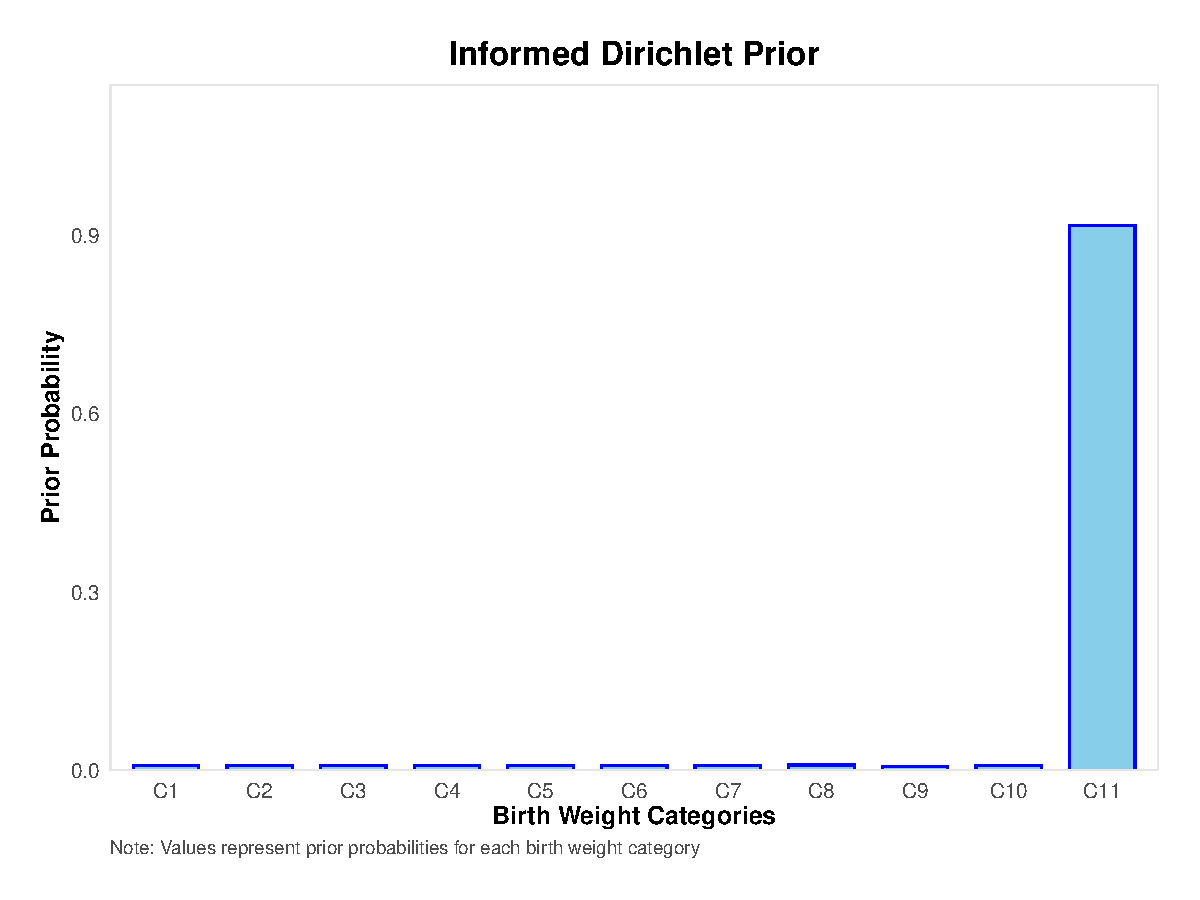
\includegraphics[width=\linewidth]{plots/alphavec_plot_2020_full.pdf}\\[-1ex]
  {\footnotesize Full model prior: LBW + NBW}
\end{minipage}
\hfill
\begin{minipage}{0.46\linewidth}
  \centering
  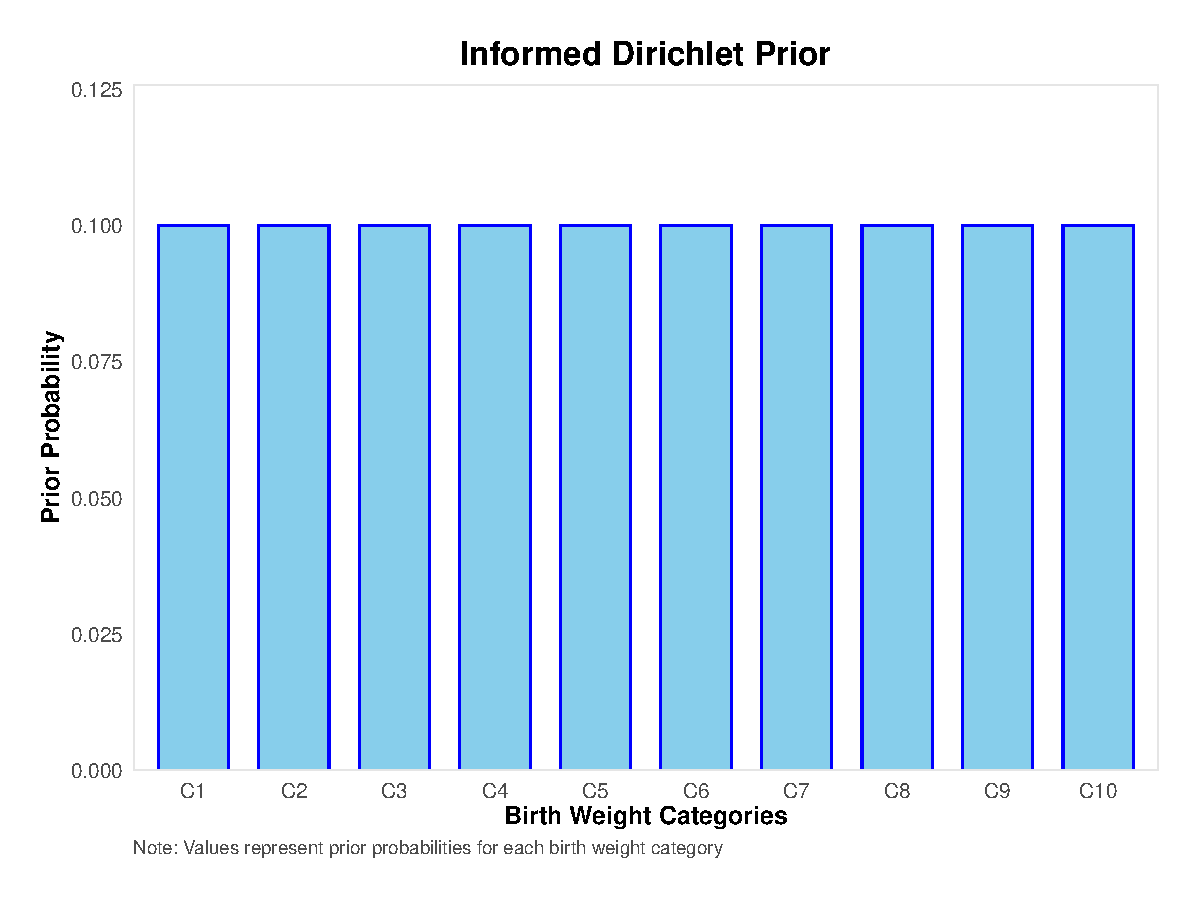
\includegraphics[width=\linewidth]{plots/alphavec_plot_2020_small.pdf}\\[-1ex]
  {\footnotesize LBW‑only prior: LBW}
\end{minipage}

\vspace{4pt}
\small Comparison of informed Dirichlet hyperparameters (2020 quantiles)
\end{frame}

% =========================================================
\section{Dirichlet–Multinomial Criterion}

% ---------- FRAME 1 : motivation + model ---------------
\begin{frame}{From Multinomial Counts to a DM Node Model}
\footnotesize         % keeps text readable & compact
\begin{columns}[T]
% ---- left column : hierarchy picture ----
\column{0.54\linewidth}
\begin{align*}  
    \mathbf x_i = &\text{ dummy-encoded predictor vec. for class } i, \\
    \mathbf y_i \;\Big|\; \boldsymbol\theta_i, \mathbf{x}_i
          &\sim \text{Adj.Multinomial}(N_i,\boldsymbol\theta_i = (\theta_{i,1}, \dots, \theta_{i,K}))\\
    \boldsymbol\theta_i \;\Big|\; \boldsymbol{\alpha} \;&\sim\;
    \text{Dirichlet}(\alpha_1, \dots, \alpha_K) \quad \text{(prior)}\\
    \boldsymbol\theta_i \;\Big|\; \mathbf{y}_i, \mathbf{x}_i \;&\sim\;
    \text{Dirichlet}(\boldsymbol\alpha + \mathbf{y}_i) \quad \text{(posterior)}
\end{align*}

\vskip2pt
\begin{itemize}
  \item Each terminal node's count vector $\mathbf y_i=(n_{i1},\dots,n_{iK})_{K \times 1}$ across $K$ weight bins for \(i=1,\dots,128\) rows.
  \item Dirichlet prior adds \emph{pseudo-counts} $\alpha_k$ to smooth zero cells \citep{poole_mackworth2025pseudo}.
  \item Use conjugacy $\Rightarrow$ closed‑form node evidence used as impurity.
\end{itemize}

% ---- right column : why we omit the multinomial coeff ----
\column{0.50\linewidth}
\textbf{Why drop the multinomial coefficient?}
\begin{itemize}\itemsep1.5pt
  \item For a split $N=N_1 + N_2$, the coefficient $\displaystyle\binom{N}{n_1,\dots,n_K} > \binom{N_1}{\cdot} + \binom{N_2}{\cdot}$ no matter the counts.
  \item If kept, CART would favor \emph{larger} partitions, not purer ones.
  \item Omitting it lets the criterion model solely the distributional fit.
\end{itemize}
\end{columns}
\end{frame}


% ---------- FRAME 2 : derivation sketch ------------------
\begin{frame}{Derivation of DM Likelihood — Key Steps}
\scriptsize
\setlength{\abovedisplayskip}{4pt}
\setlength{\belowdisplayskip}{4pt}

\textbf{1.  Joint density}\par
\begin{align*}
    p(\mathbf y,\boldsymbol\theta \mid \mathbf x) 
    \;&=\; 
    p(\mathbf{y} \mid \boldsymbol{\theta}, \mathbf{x}) p(\boldsymbol{\theta})
    \;=\; \underbrace{\prod_{k=1}^K\theta_k^{n_k}}_{\mathrm{Adj.Multinomial}} 
    \underbrace{\frac{1}{B(\boldsymbol\alpha)} \cdot
    \prod_{k=1}^K\theta_k^{\alpha_k-1}}_{\mathrm{Dirichlet}}
    = \frac{\Gamma(\alpha_0)}{\prod_k\Gamma(\alpha_k)}
      \prod_{k=1}^K\theta_k^{n_k+\alpha_k-1}\\
    &\propto \prod_{k=1}^K \theta_k^{(n_k+\alpha_k)-1} \sim \mathrm{Dirichlet}(\boldsymbol\alpha + \mathbf{y})
\end{align*}


\textbf{2.  Integrate out $\boldsymbol\theta$}\par
\[
    p(\mathbf y\mid\boldsymbol\alpha, \mathbf{x})
    \;=\; 
    \int_{\boldsymbol{\theta}} p(\mathbf y,\boldsymbol\theta)\,d\boldsymbol\theta
    \;=\; 
    \frac{\Gamma(\alpha_0)}{\prod_k\Gamma(\alpha_k)}
        \,B(\mathbf y+\boldsymbol\alpha)
    \;=\; 
    \frac{\Gamma(\alpha_0)} {\Gamma(N+\alpha_0)}
    \left( \prod_{k=1}^K\frac{\Gamma(n_k+\alpha_k)}{\Gamma(\alpha_k)} \right)
\]

\textbf{3.  Log-likelihood (used as node deviance)}\par
\[
\ell = \log p(\mathbf{y} \mid \boldsymbol{\alpha},\mathbf{x}) =\log\Gamma(\alpha_0)-\log\Gamma(N+\alpha_0) + \sum_{k=1}^K\bigl[\log\Gamma(n_k+\alpha_k)-\log\Gamma(\alpha_k)\bigr].
\]

\textbf{4.  Split gain}\quad
$\displaystyle\Delta\ell=\ell_{\text{left}}+\ell_{\text{right}}-\ell_{\text{parent}}$.\par
\medskip
\tiny
(based on \citealp{mimno_polya,gundersen2020dirichlet-multinomial,minka2000estimating})
\end{frame}
%=========================================================

% -------------------------------------------------------
\section{Decision Trees}

% 1 ──────────────────────────────────────────────────────

\begin{frame}{DM–CART Construction}
\begin{enumerate}
  \item Compute $\Delta\ell$ for every candidate split.
  \item Pick the largest positive gain; recurse until no gain or max depth.
  \item Fit two trees: (i) full (LBW + NBW) and (ii) LBW‑only.
\end{enumerate}
{\footnotesize Using \texttt{rpart}\;\citep{intro_to_rpart,rpart_docs}.}
\end{frame}

% 2 ──────────────────────────────────────────────────────
\begin{frame}{\emph{Full Model} Tree Structure}
\footnotesize
\begin{columns}[T]  % top aligned
% ---- picture ----
\column{0.60\linewidth}
\centering
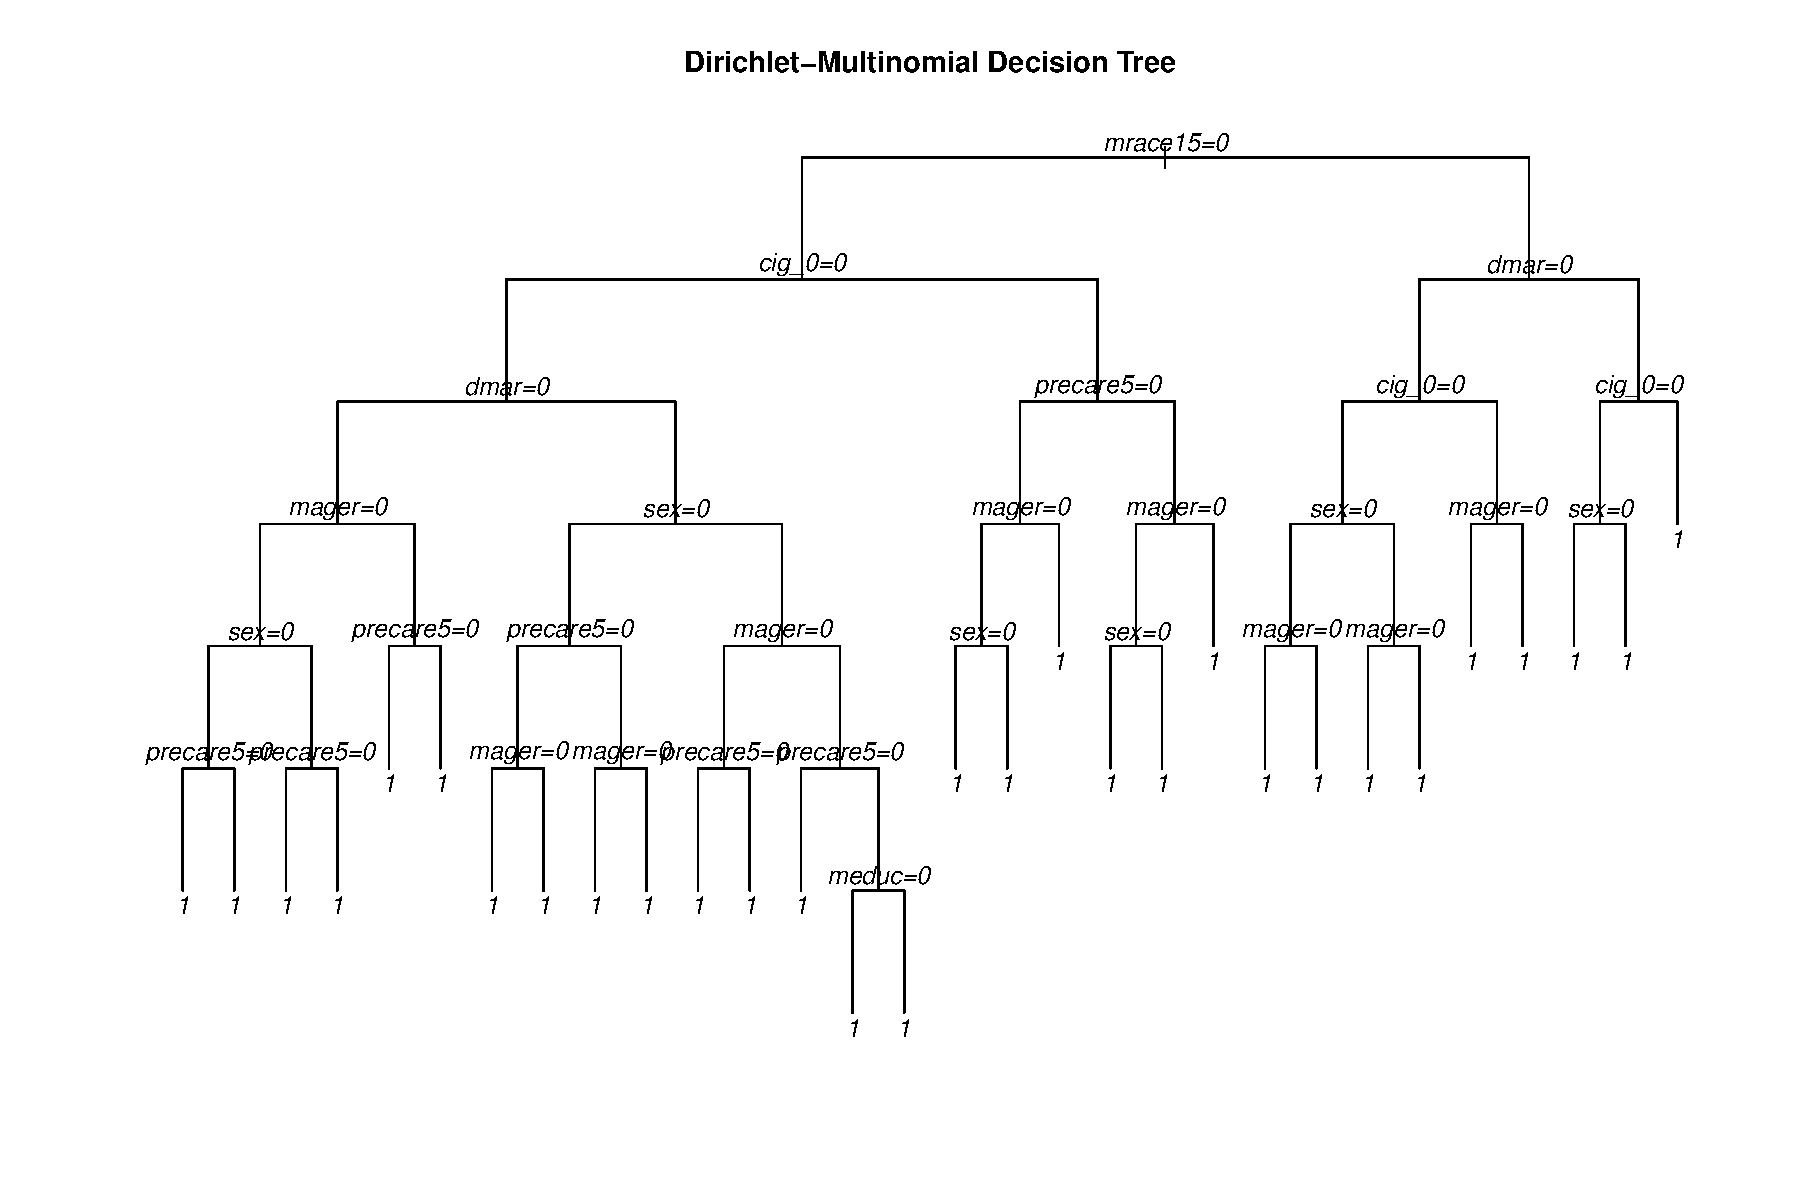
\includegraphics[height=0.75\textheight,keepaspectratio]{plots/dm_tree2021.pdf}

% ---- bullets ----
\column{0.40\linewidth}
\begin{itemize}\itemsep2pt
  \item \textbf{Root split:} maternal race (Black vs non-Black) – biggest deviance drop.
  \item Next: smoking status, then marital status.
  \item Model focus: socioeconomic/demographic
\end{itemize}
\end{columns}
\end{frame}


% 3 ──────────────────────────────────────────────────────
\begin{frame}{\emph{LBW-only Model} Tree Structure}
\footnotesize
\begin{columns}[T]
\column{0.60\linewidth}
\centering
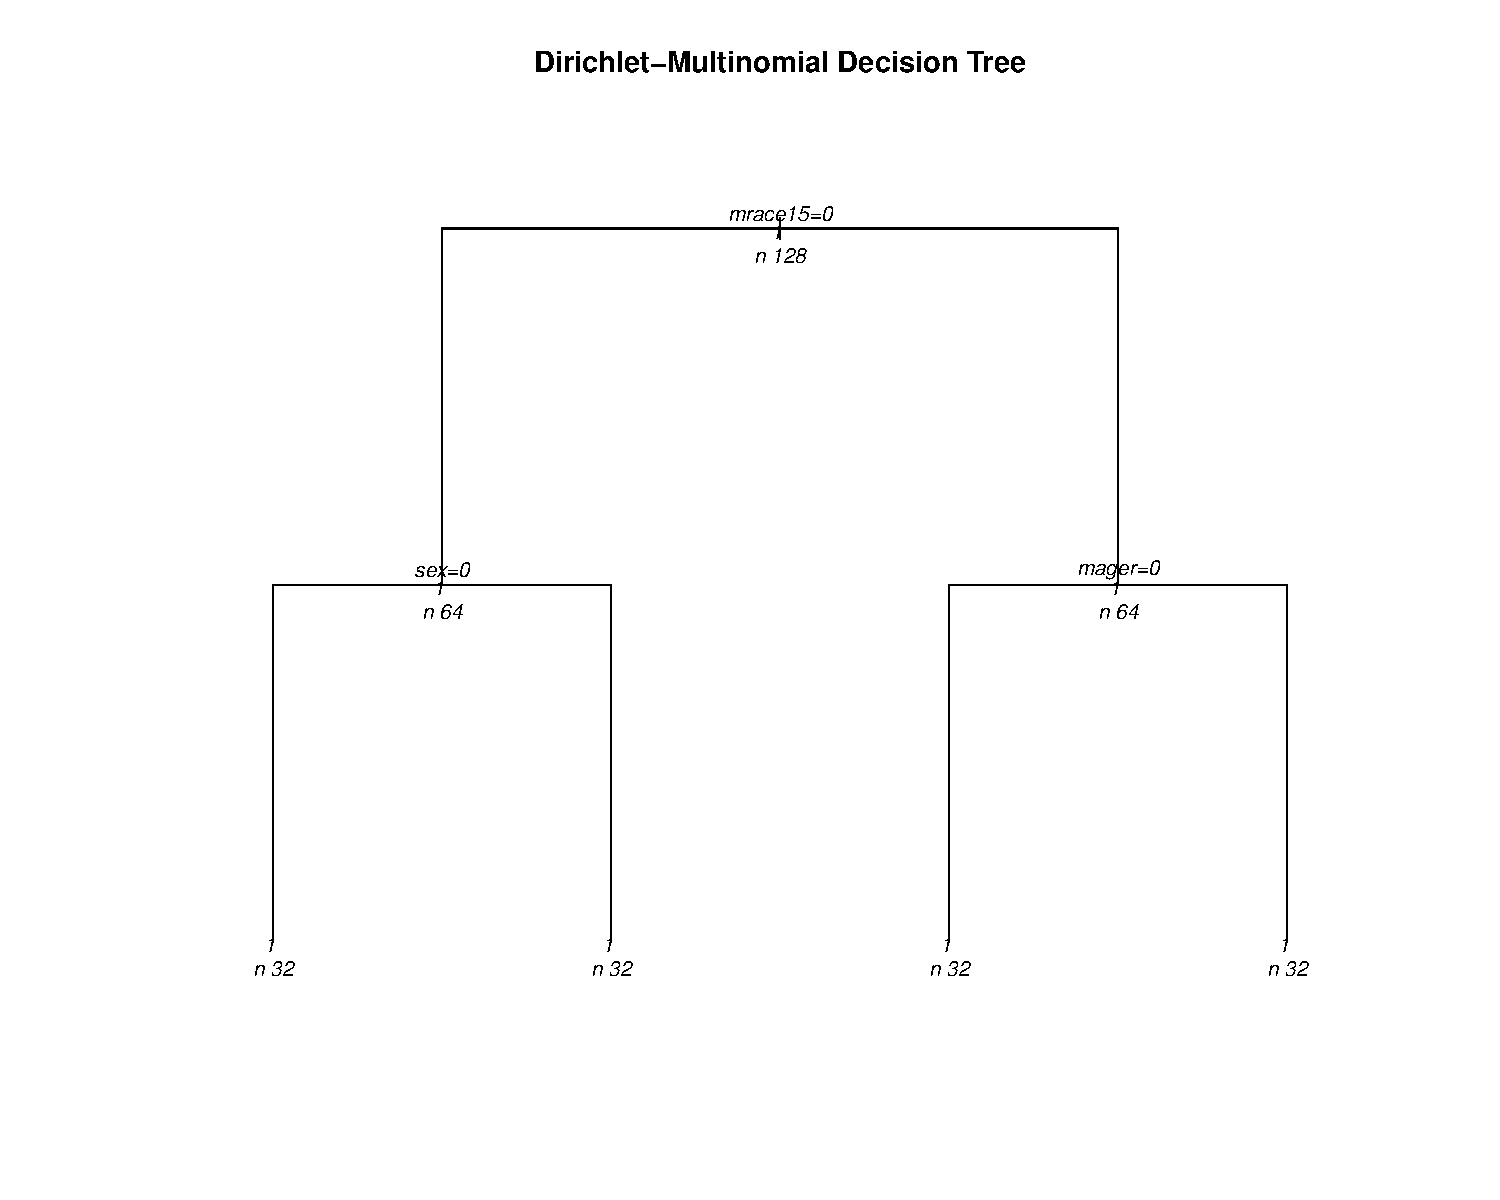
\includegraphics[height=0.75\textheight,keepaspectratio]{plots/dm_tree2021_2.pdf}

\column{0.40\linewidth}
\begin{itemize}\itemsep2pt
  \item Race still dominates the root.
  \item Race, infant sex, and maternal age are the only considered predictors.
  \item Model focus: biological/genetic
\end{itemize}
\end{columns}
\end{frame}

%================================================================
\section{Depth-Controlled Model Comparison}


%---------------------------------------------------------------
% helper: tiny 2×2 grid of depth-plots --------------------------
\newcommand{\DepthGrid}[1]{%   #1 = folder name
  \begin{tabular}{@{}cc@{}}
      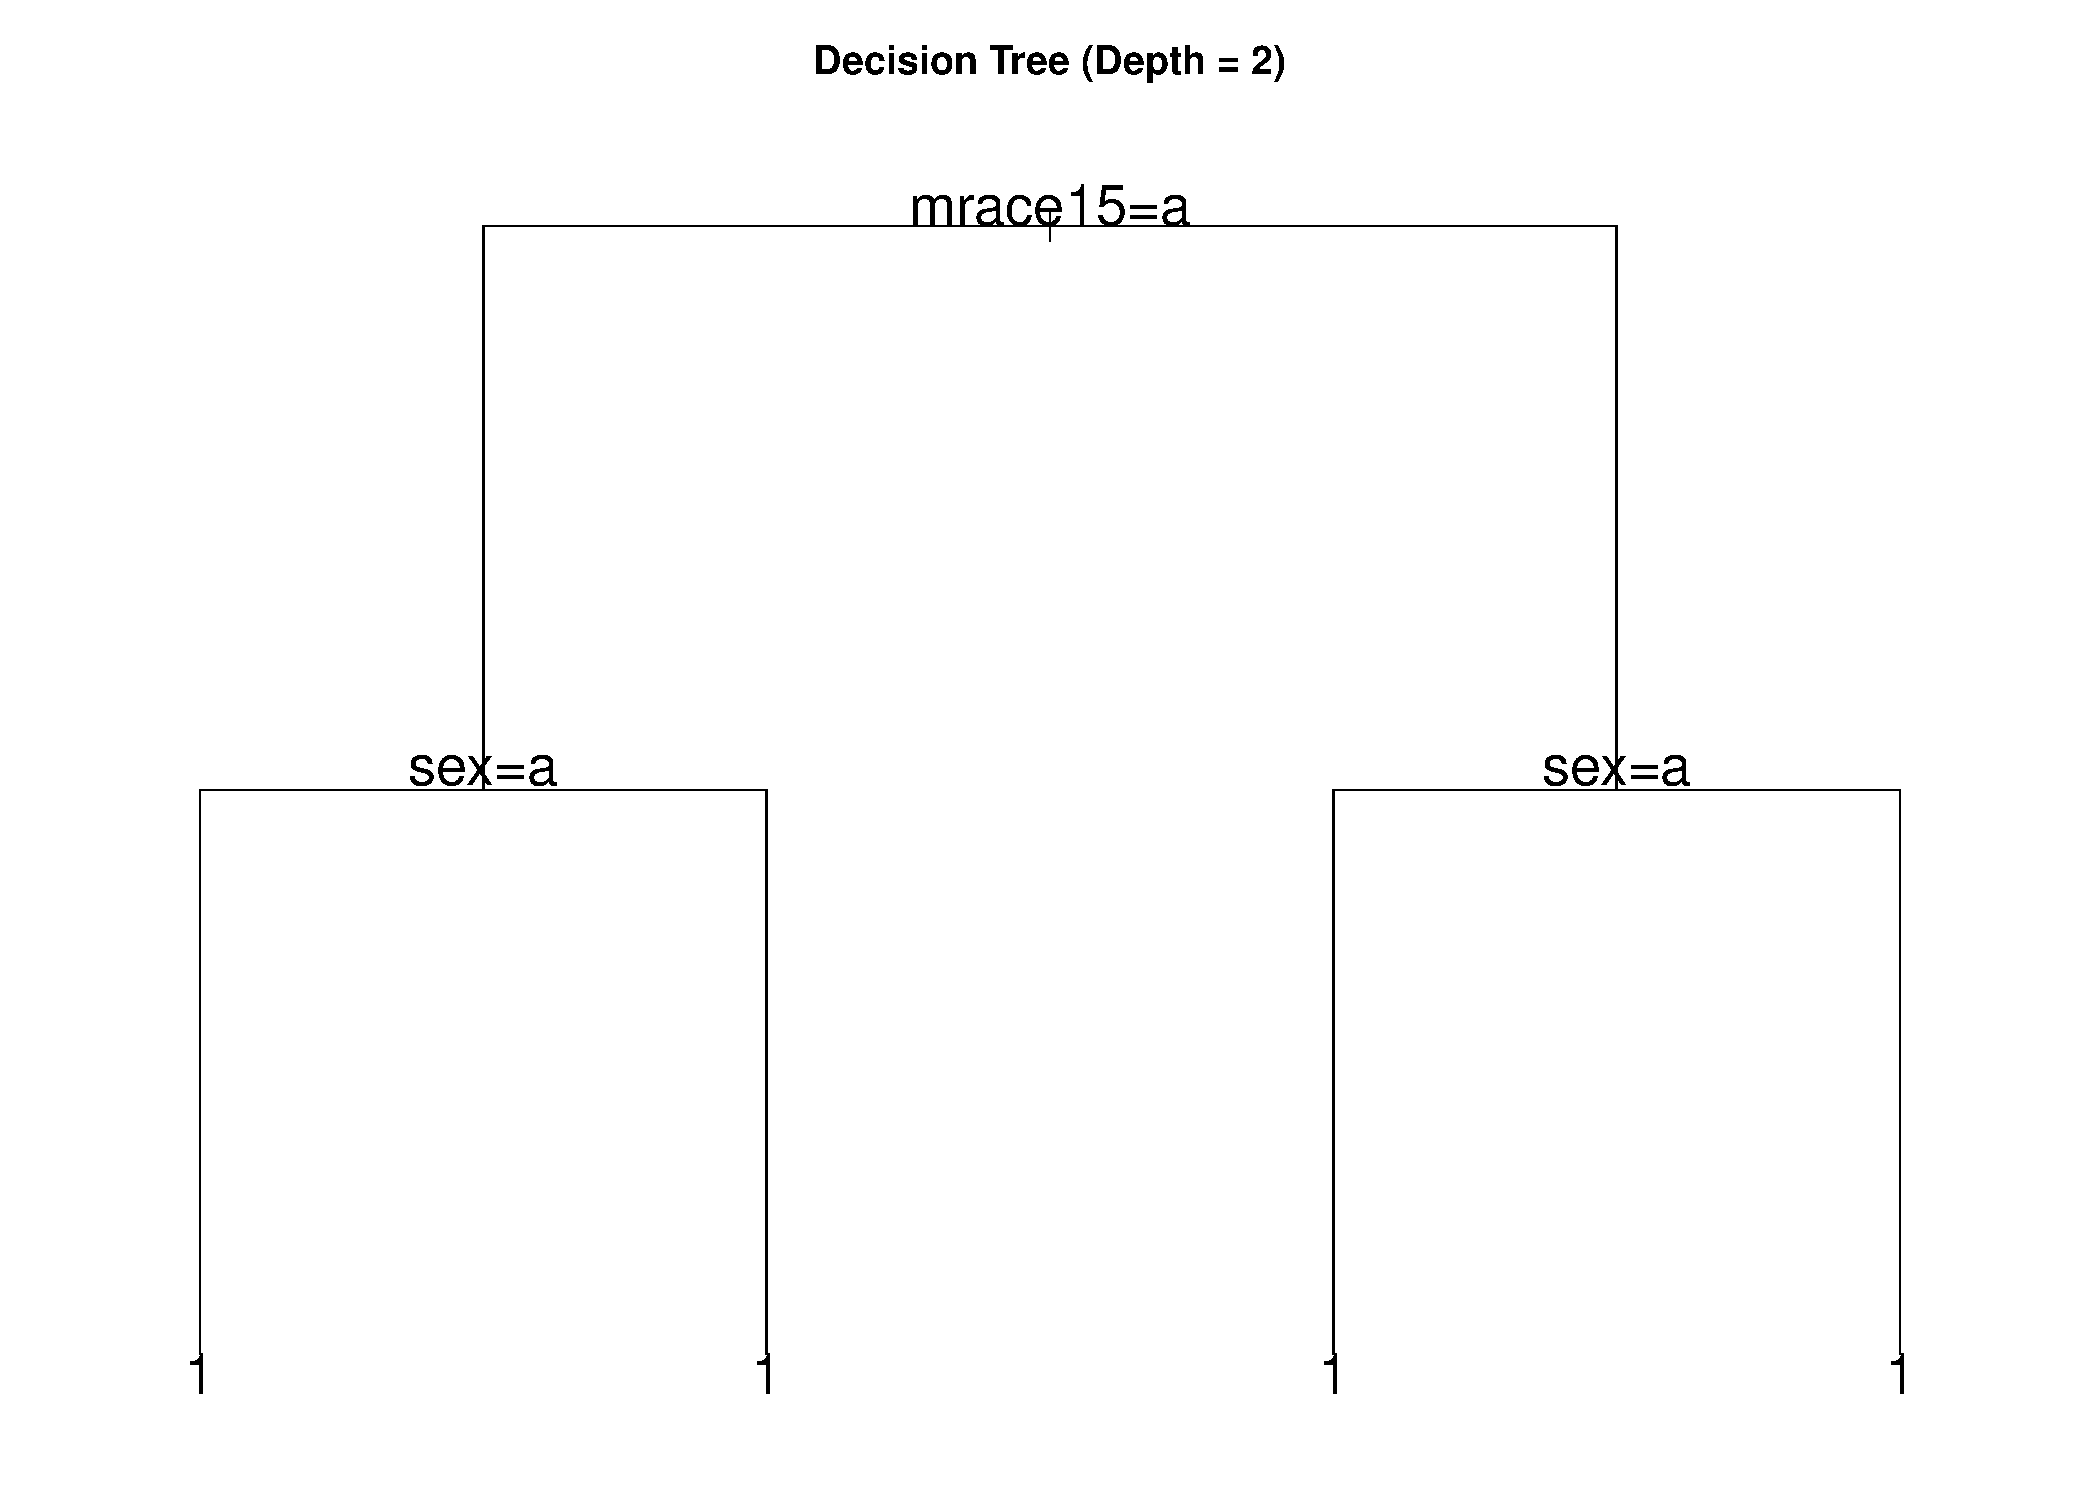
\includegraphics[trim=20 10 20 10,clip,
                       height=.35\textheight]{plots/#1/decision_tree_depth_2.pdf} &
      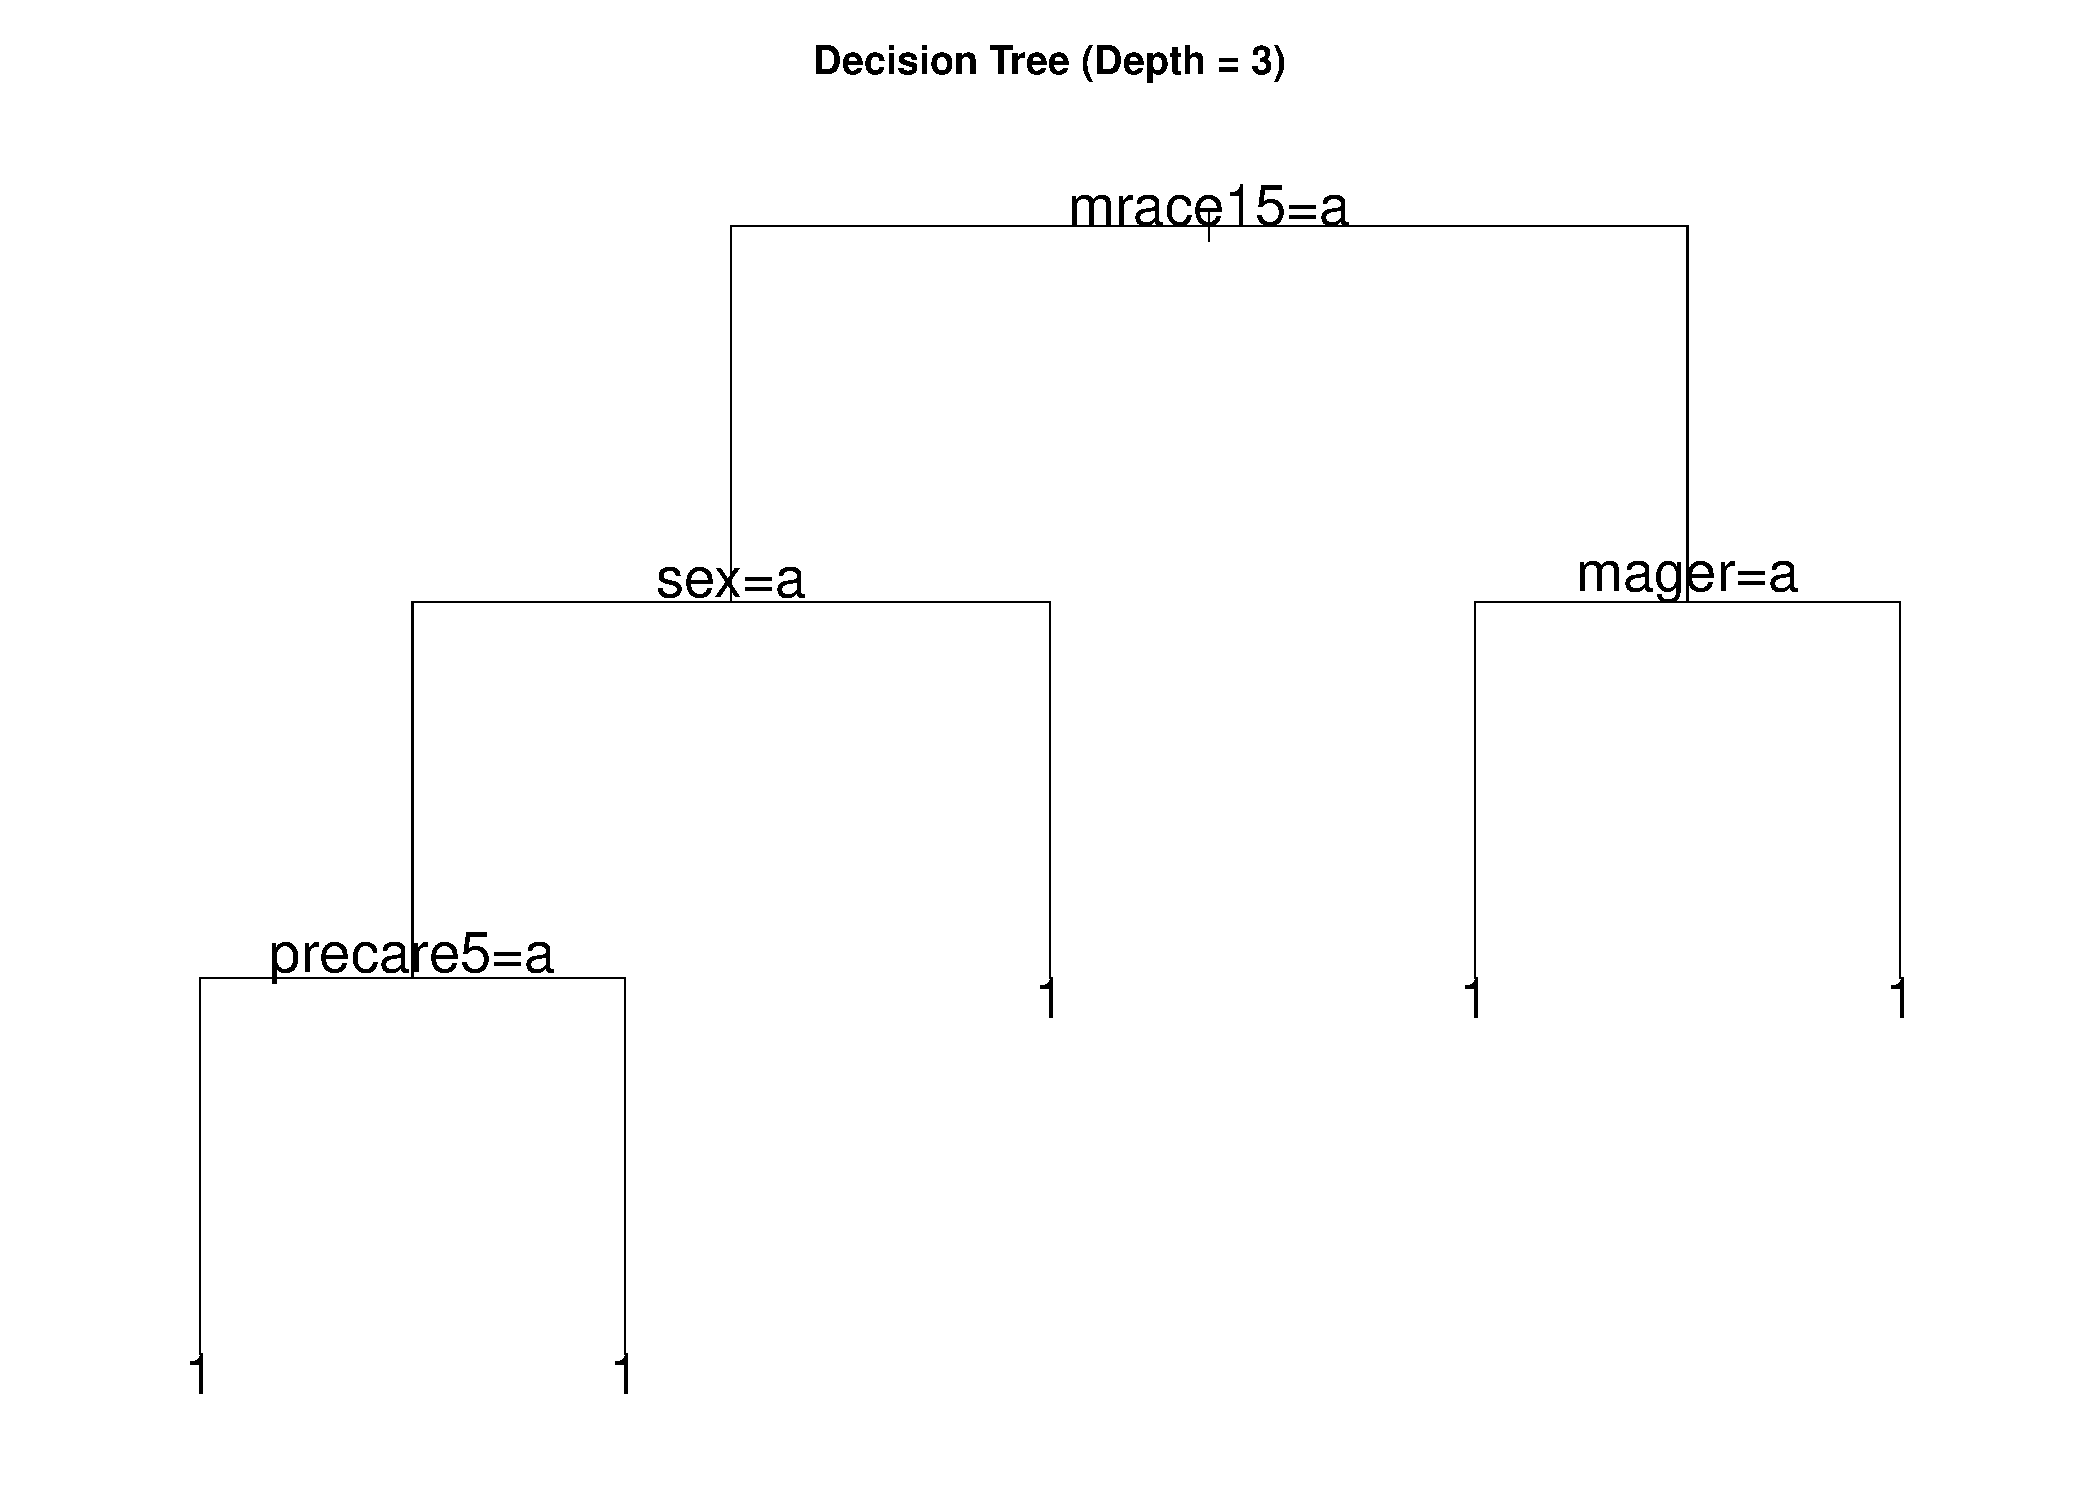
\includegraphics[trim=20 10 20 10,clip,
                       height=.35\textheight]{plots/#1/decision_tree_depth_3.pdf}\\[-4pt]
      {\tiny depth = 2} & {\tiny depth = 3}\\[2pt]
      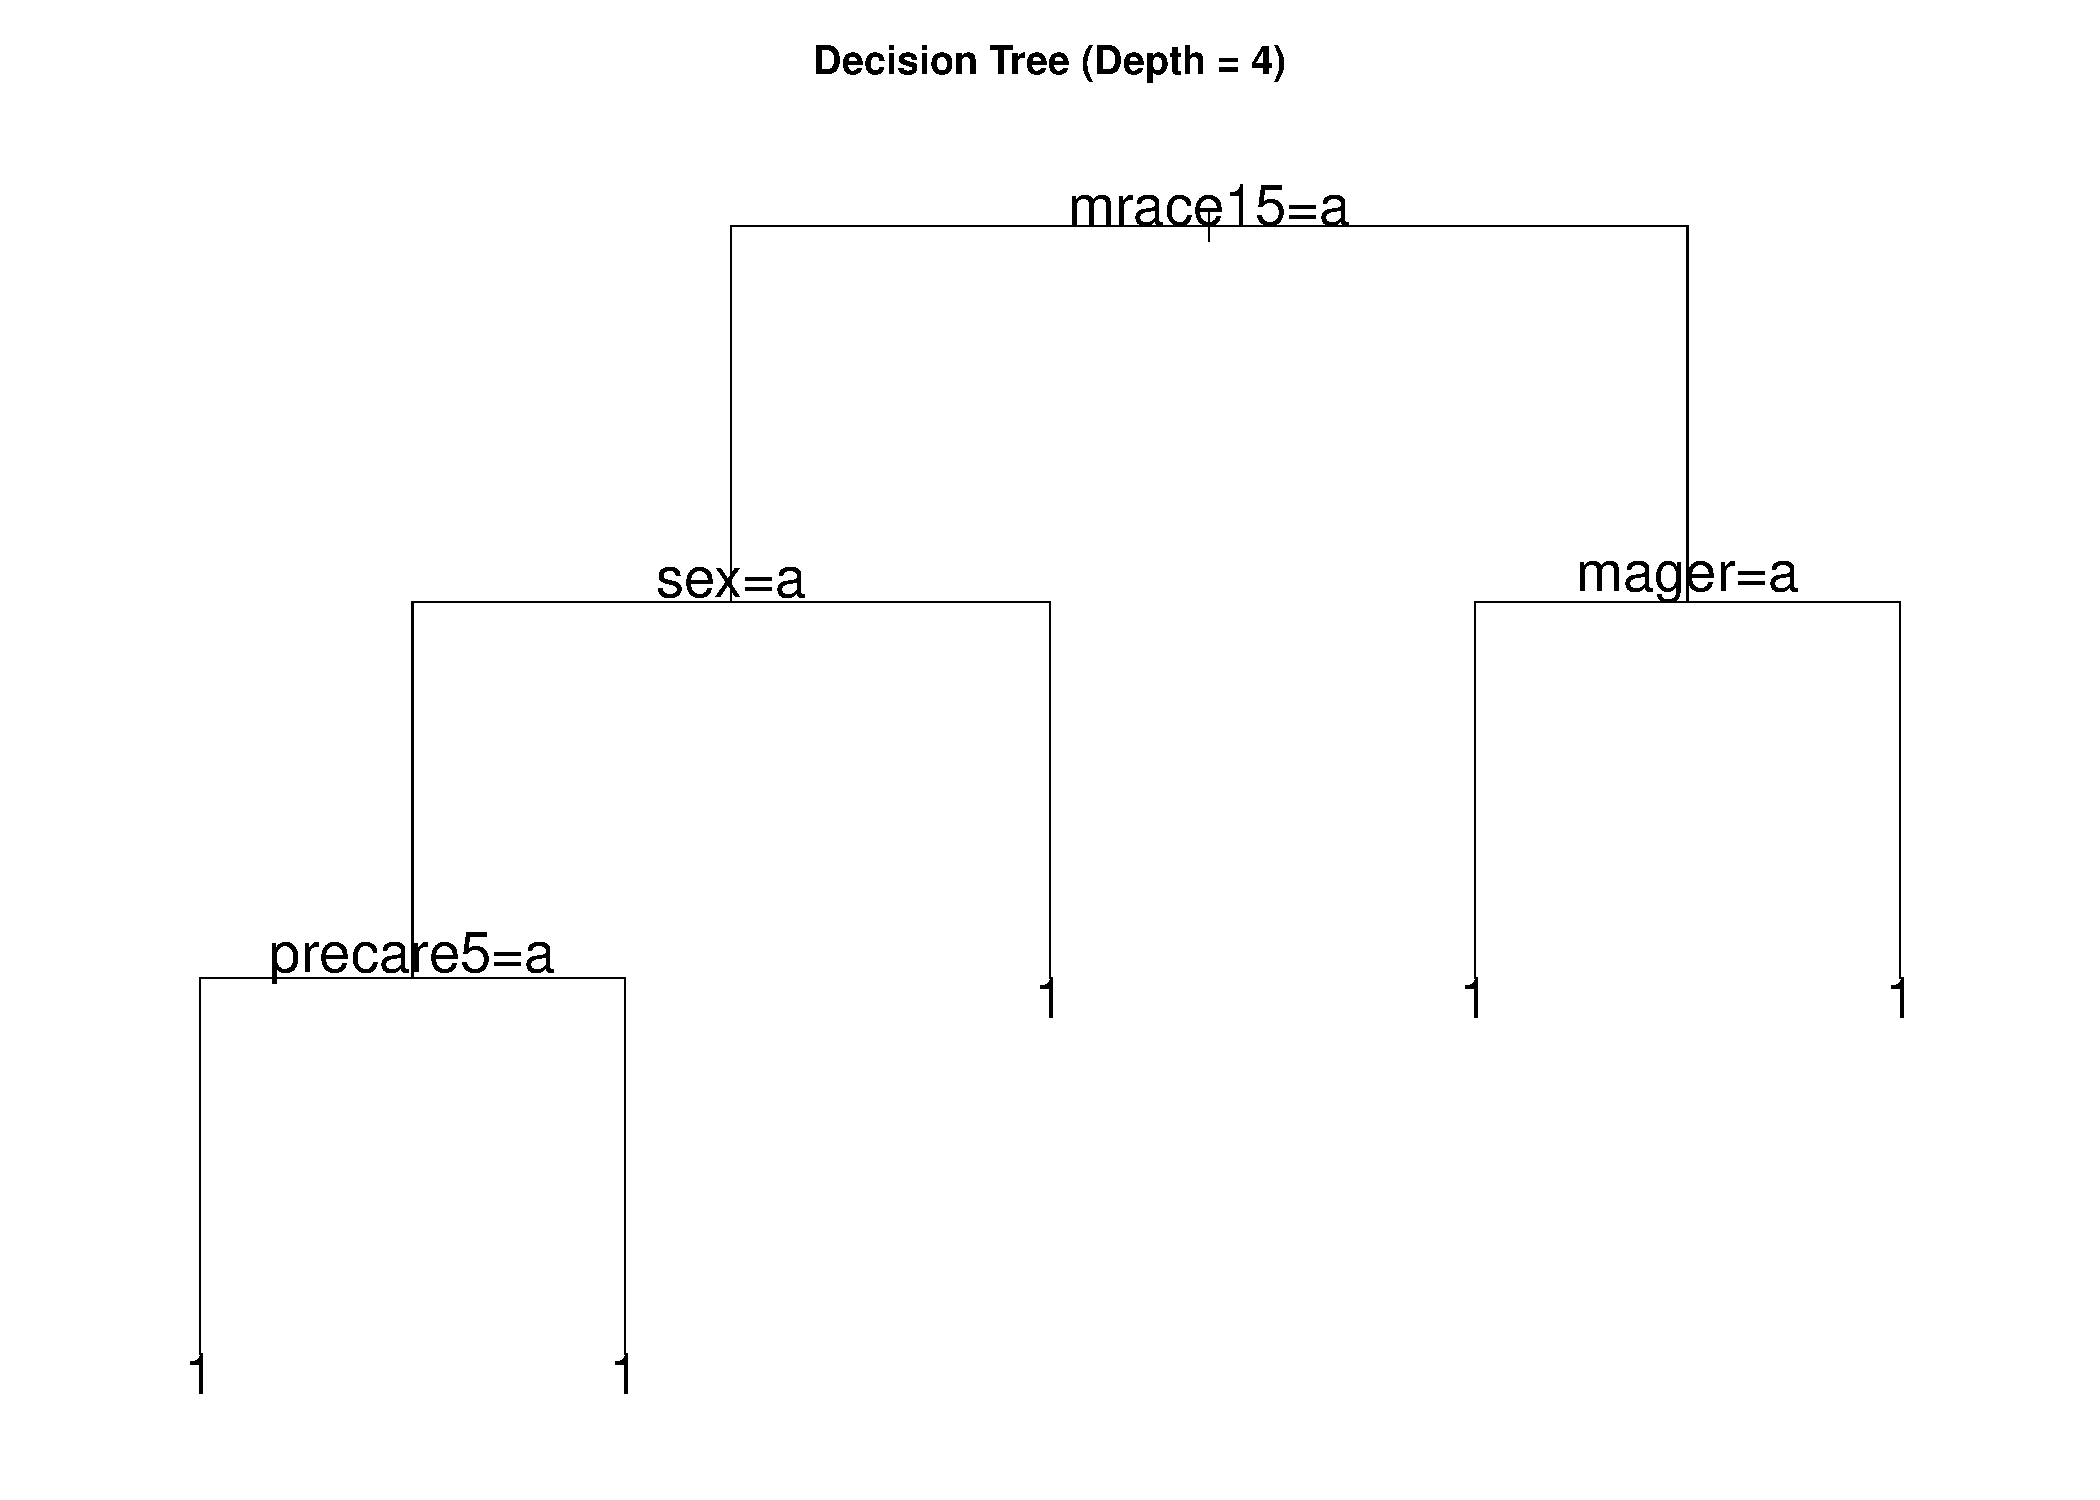
\includegraphics[trim=20 10 20 10,clip,
                       height=.35\textheight]{plots/#1/decision_tree_depth_4.pdf} &
      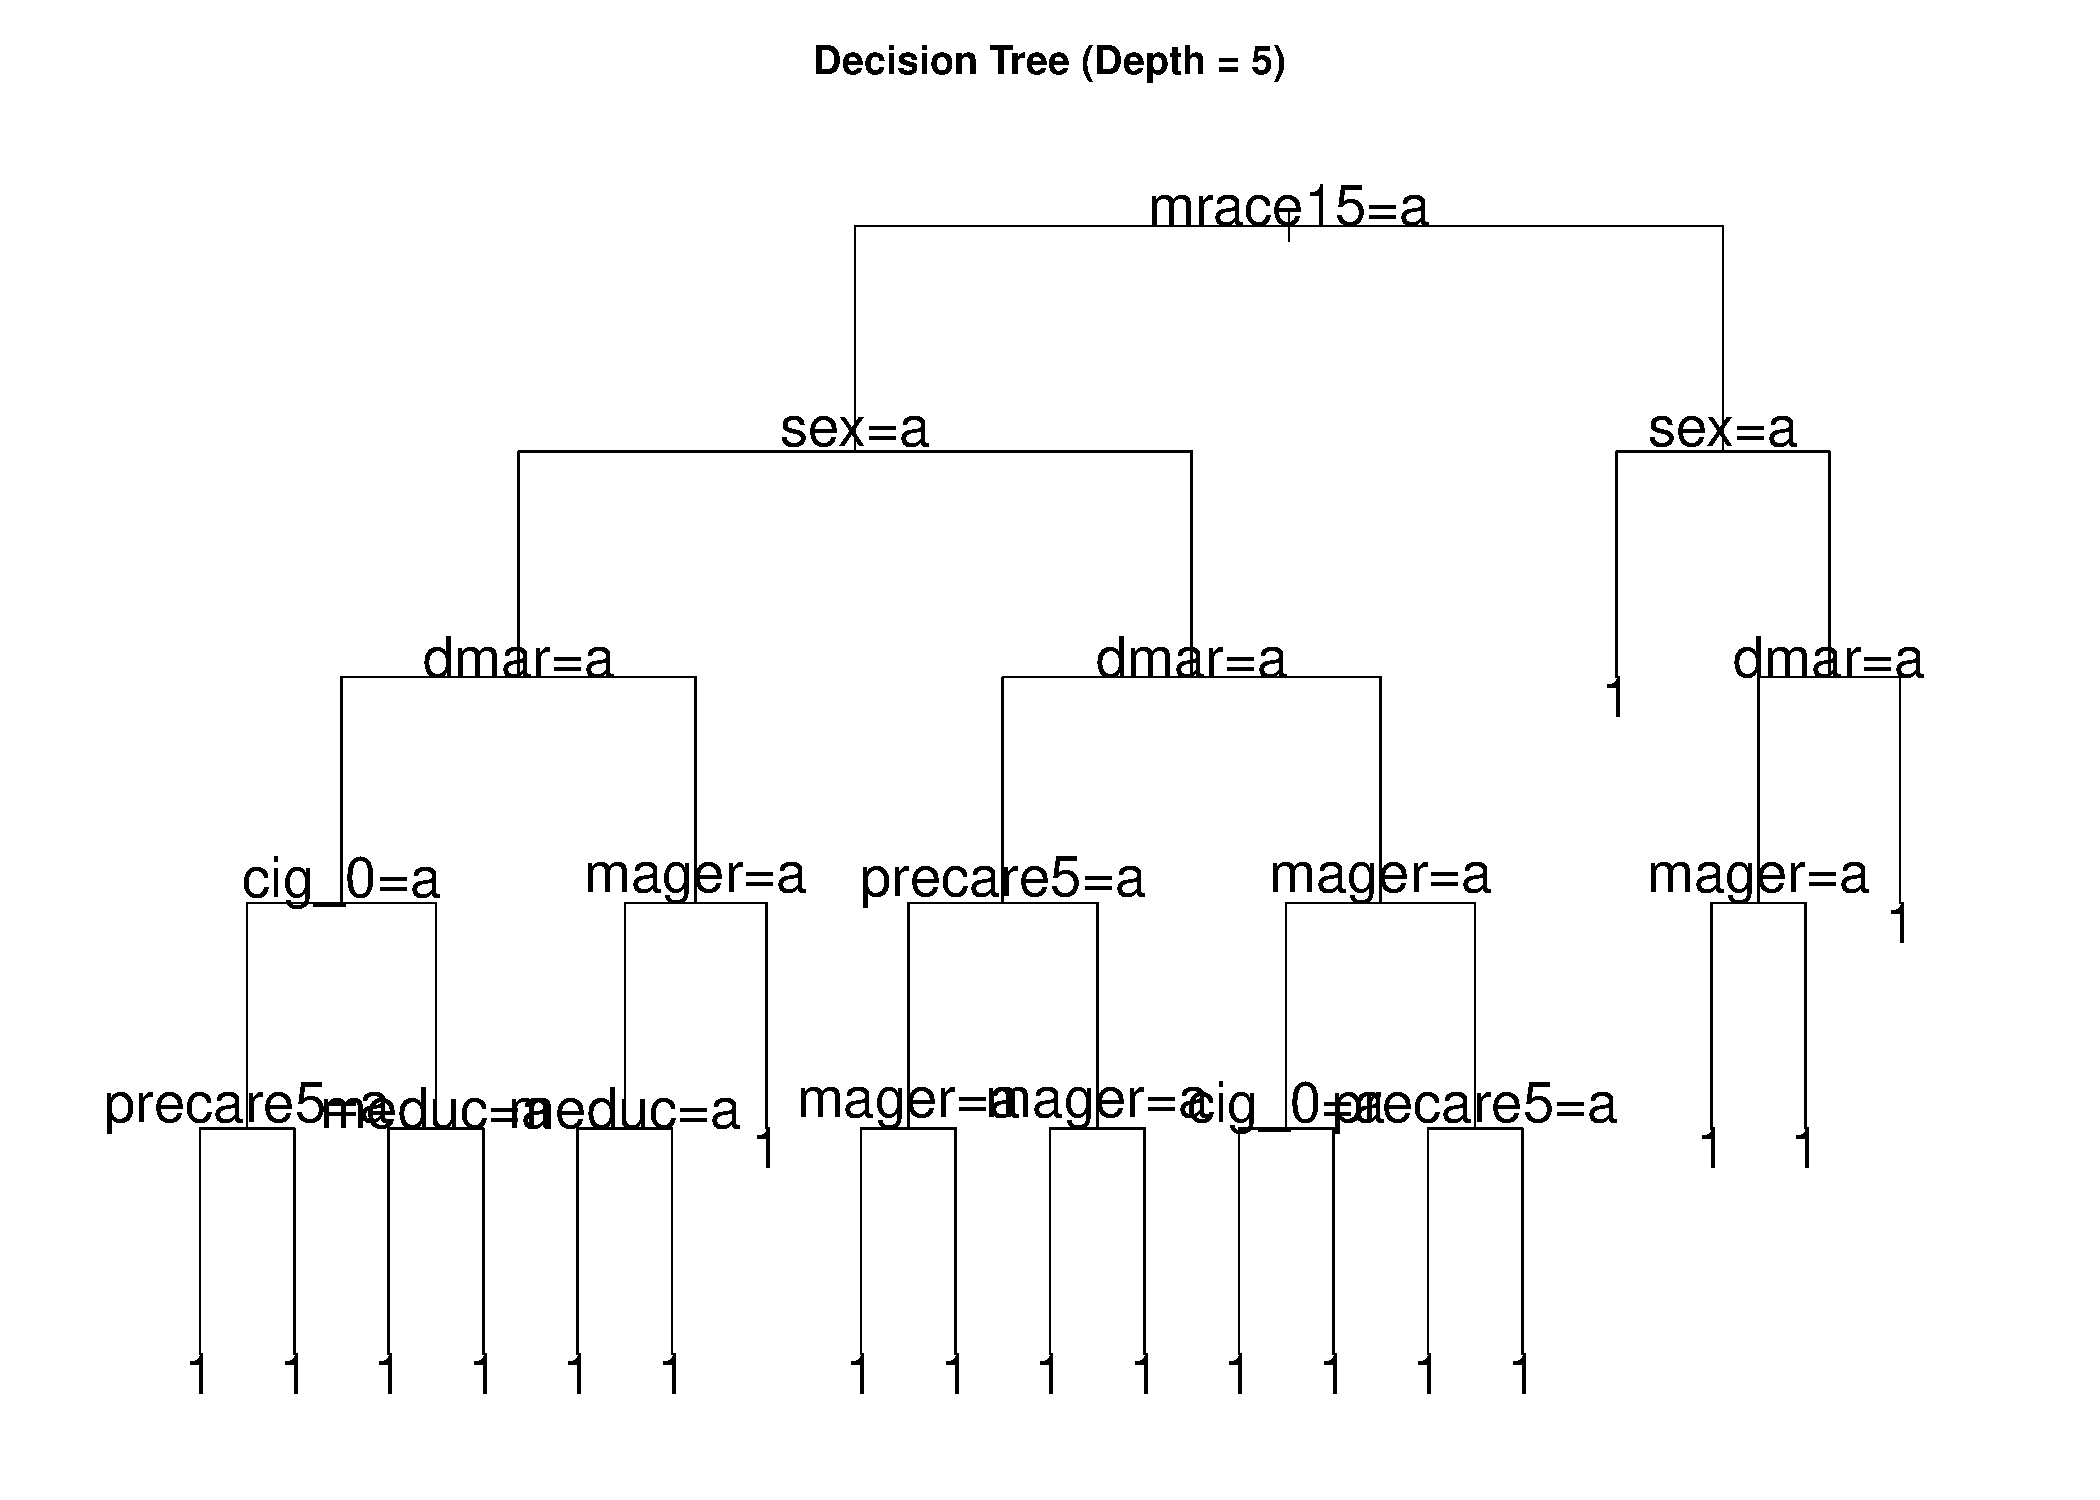
\includegraphics[trim=20 10 20 10,clip,
                       height=.35\textheight]{plots/#1/decision_tree_depth_5.pdf}\\[-4pt]
      {\tiny depth = 4} & {\tiny depth = 5}
  \end{tabular}}

%---------------------------------------------------------------
% 1) full model grid + notes
%---------------------------------------------------------------
\begin{frame}{Depth Comparison — Full Model}
\scriptsize
\begin{columns}[T]

\column{0.60\linewidth}
\centering
\DepthGrid{depth1}   % <-- plots/depth1/decision_tree_depth_X.pdf

\column{0.40\linewidth}
\begin{itemize}\itemsep2pt
  \item Terminal nodes grow from 4 → 19.
  \item Splitting order: race $\to$ sex $\to$ marital remains entirely unchanged.
  \item Interestingly, smoking appears only at depth 4. 
  \item For non-Black mothers, the branch is far more shallow than for Black mothers.
\end{itemize}

\end{columns}
\end{frame}

%---------------------------------------------------------------
% 2) LBW-only grid + notes
%---------------------------------------------------------------
\begin{frame}{Depth Comparison — LBW-Only Model}
\scriptsize
\begin{columns}[T]

\column{0.60\linewidth}
\centering
\DepthGrid{depth2}   % <-- plots/depth2/decision_tree_depth_X.pdf

\column{0.40\linewidth}
\begin{itemize}\itemsep2pt
    \item Terminal nodes grow from 4 → 5, much shallower.  
    \item Race still opens every tree.
    \item Splitting order: infant gender, maternal age, then prenatal care. Improvement stagnates quickly with restricted LBW data.
  \item Smoking \emph{never} included. 
\end{itemize}

\end{columns}
\end{frame}


% =========================================================
\section{Bootstrap Ensemble}
\begin{frame}{Two‑Tier Parametric Bootstrap Methodology (\(B = 10,000\))}
\footnotesize
Notation: \(T=\sum_i \sum_k n_{ik}\) (grand total), \(N_i = \sum_k^K n_{i,k}\) (class total) and \(p_i = N_i/T\) (empirical class shares).
% For \(B = 10,000\) bootstrap replicates, 

\textbf{Tier 1 — Between‑class counts resampling}\par
Draw a new vector of class totals, once per class, \emph{propagating prevalence of \(N\) profiles}.
\[
  \mathbf{n}^\ast = (n_1^{\ast},\dots,n_{N}^{\ast}) \;\sim\; \operatorname{Multinomial}\bigl(T,\,\mathbf p\bigr), \quad i = 1,\dots, N=128
\]

\textbf{Tier 2 — Within‑class counts resampling}\par
Given new \(n_i^{\ast}>0\), resample \(K\) category counts:
\[
  \tilde{\mathbf{y}}_i = (\tilde n_{i,1},\dots,\tilde n_{i,K})
  \;\sim\; \operatorname{Multinomial}\bigl(n_i^{\ast},\,\hat{\boldsymbol\pi}_i\bigr), \quad \text{where } \hat{\boldsymbol{\pi}}_i  = (\hat{\pi}_{i,1}, \dots, \hat{\pi}_{i,K})
\]

\(\hat{\pi}_{i,k} = (n_{ik}+\alpha_k)/(N_i + \alpha_0)\) held \emph{fixed} during resampling (focusing on observed counts variability).

\(\hat{\boldsymbol\pi}_i\) are the \emph{mean bootstrap probability estimates} for \(K\) birth-weight categories across \(B\) replicates. Interpreted as the best guess of a future birth of class \(i\) to fall into category \(k\).

\(\mathbb{E}[\tilde{\mathbf{y}}_i] = n_i^\ast \hat{\pi}_{i,k} \)
are the \emph{expected counts} for category \(k\) in class \(i\), centered around \(\boldsymbol{\pi}_i\).


\end{frame}


% % =========================================================
\begin{frame}{Interpreting the Ensemble}
\begin{itemize}
  \item Each bootstrap tree is fitted to the resampled \(\tilde{\mathbf Y}\) with DM‑CART.
  \item For every predictor we record:
        \begin{itemize}
          \item \textbf{Variable-Inclusion percent}: proportion of trees where the variable appears (any depth).
          \item \textbf{Root‑split percent}: proportion of trees where variable is used as root split.
        \end{itemize}
  \item Proportions show predictors importance under each scope using the DM-CART method.
  \item We also aggregate \(\hat{\pi}_{i,k}\) across replicates to obtain point estimates and 95\% percentile intervals for any subgroup.
  \item Contrast: \textit{high-risk} (class 69) and \textit{low-risk} (class 28) probability estimates. 
    \begin{itemize}
          \item \textit{High-risk}: unmarried, Black, smoking mother under 33 with $<$ High-School education, inadequate prenatal care, delivering female infants
          \item \textit{Low-risk}: married, non-Black, non-smoking mothers aged 33+, $\geq$ High-School education, adequate prenatal care, delivering male infants
    \end{itemize}
    
\end{itemize}
\end{frame}


\begin{frame}{Variable Importance: Full vs.\ LBW-Only Models}

\small        % shrink text a bit so the whole table fits
\centering

\begin{tabular}{@{}lcc@{}}
\toprule
                & \multicolumn{1}{c}{\textbf{Full Model}} & \multicolumn{1}{c}{\textbf{LBW-Only Model}} \\
\cmidrule(lr){2-2}\cmidrule(lr){3-3}
\multicolumn{3}{l}{\emph{Initial Split Variable}} \\
\midrule
mrace15         & 1.0000 & 1.0000 \\
\midrule
\multicolumn{3}{l}{\emph{Variable Frequency}} \\
\midrule
sex             & 1.0000 & 1.0000 \\
dmar            & 1.0000 & 0.0915 \\
mrace15         & 1.0000 & 1.0000 \\
mager           & 1.0000 & 0.9741 \\
precare5        & 1.0000 & 0.6351 \\
cig\_0          & 1.0000 & 0.0196 \\
meduc           & 0.3794 & 0.0000 \\
\bottomrule
\end{tabular}

\medskip
\scriptsize
\textit{Note:} "Variable frequency" (proportion of trees containing each variable) and

"Initial Split Variable" (normalized measure of predictive contribution) for both models.
\end{frame}


\begin{frame}{Predictor Depth Across Ensemble}
\small Histograms of predictor inclusion depth across ensemble.
\begin{columns}[T]
  \column{0.5\linewidth}
    \centering
    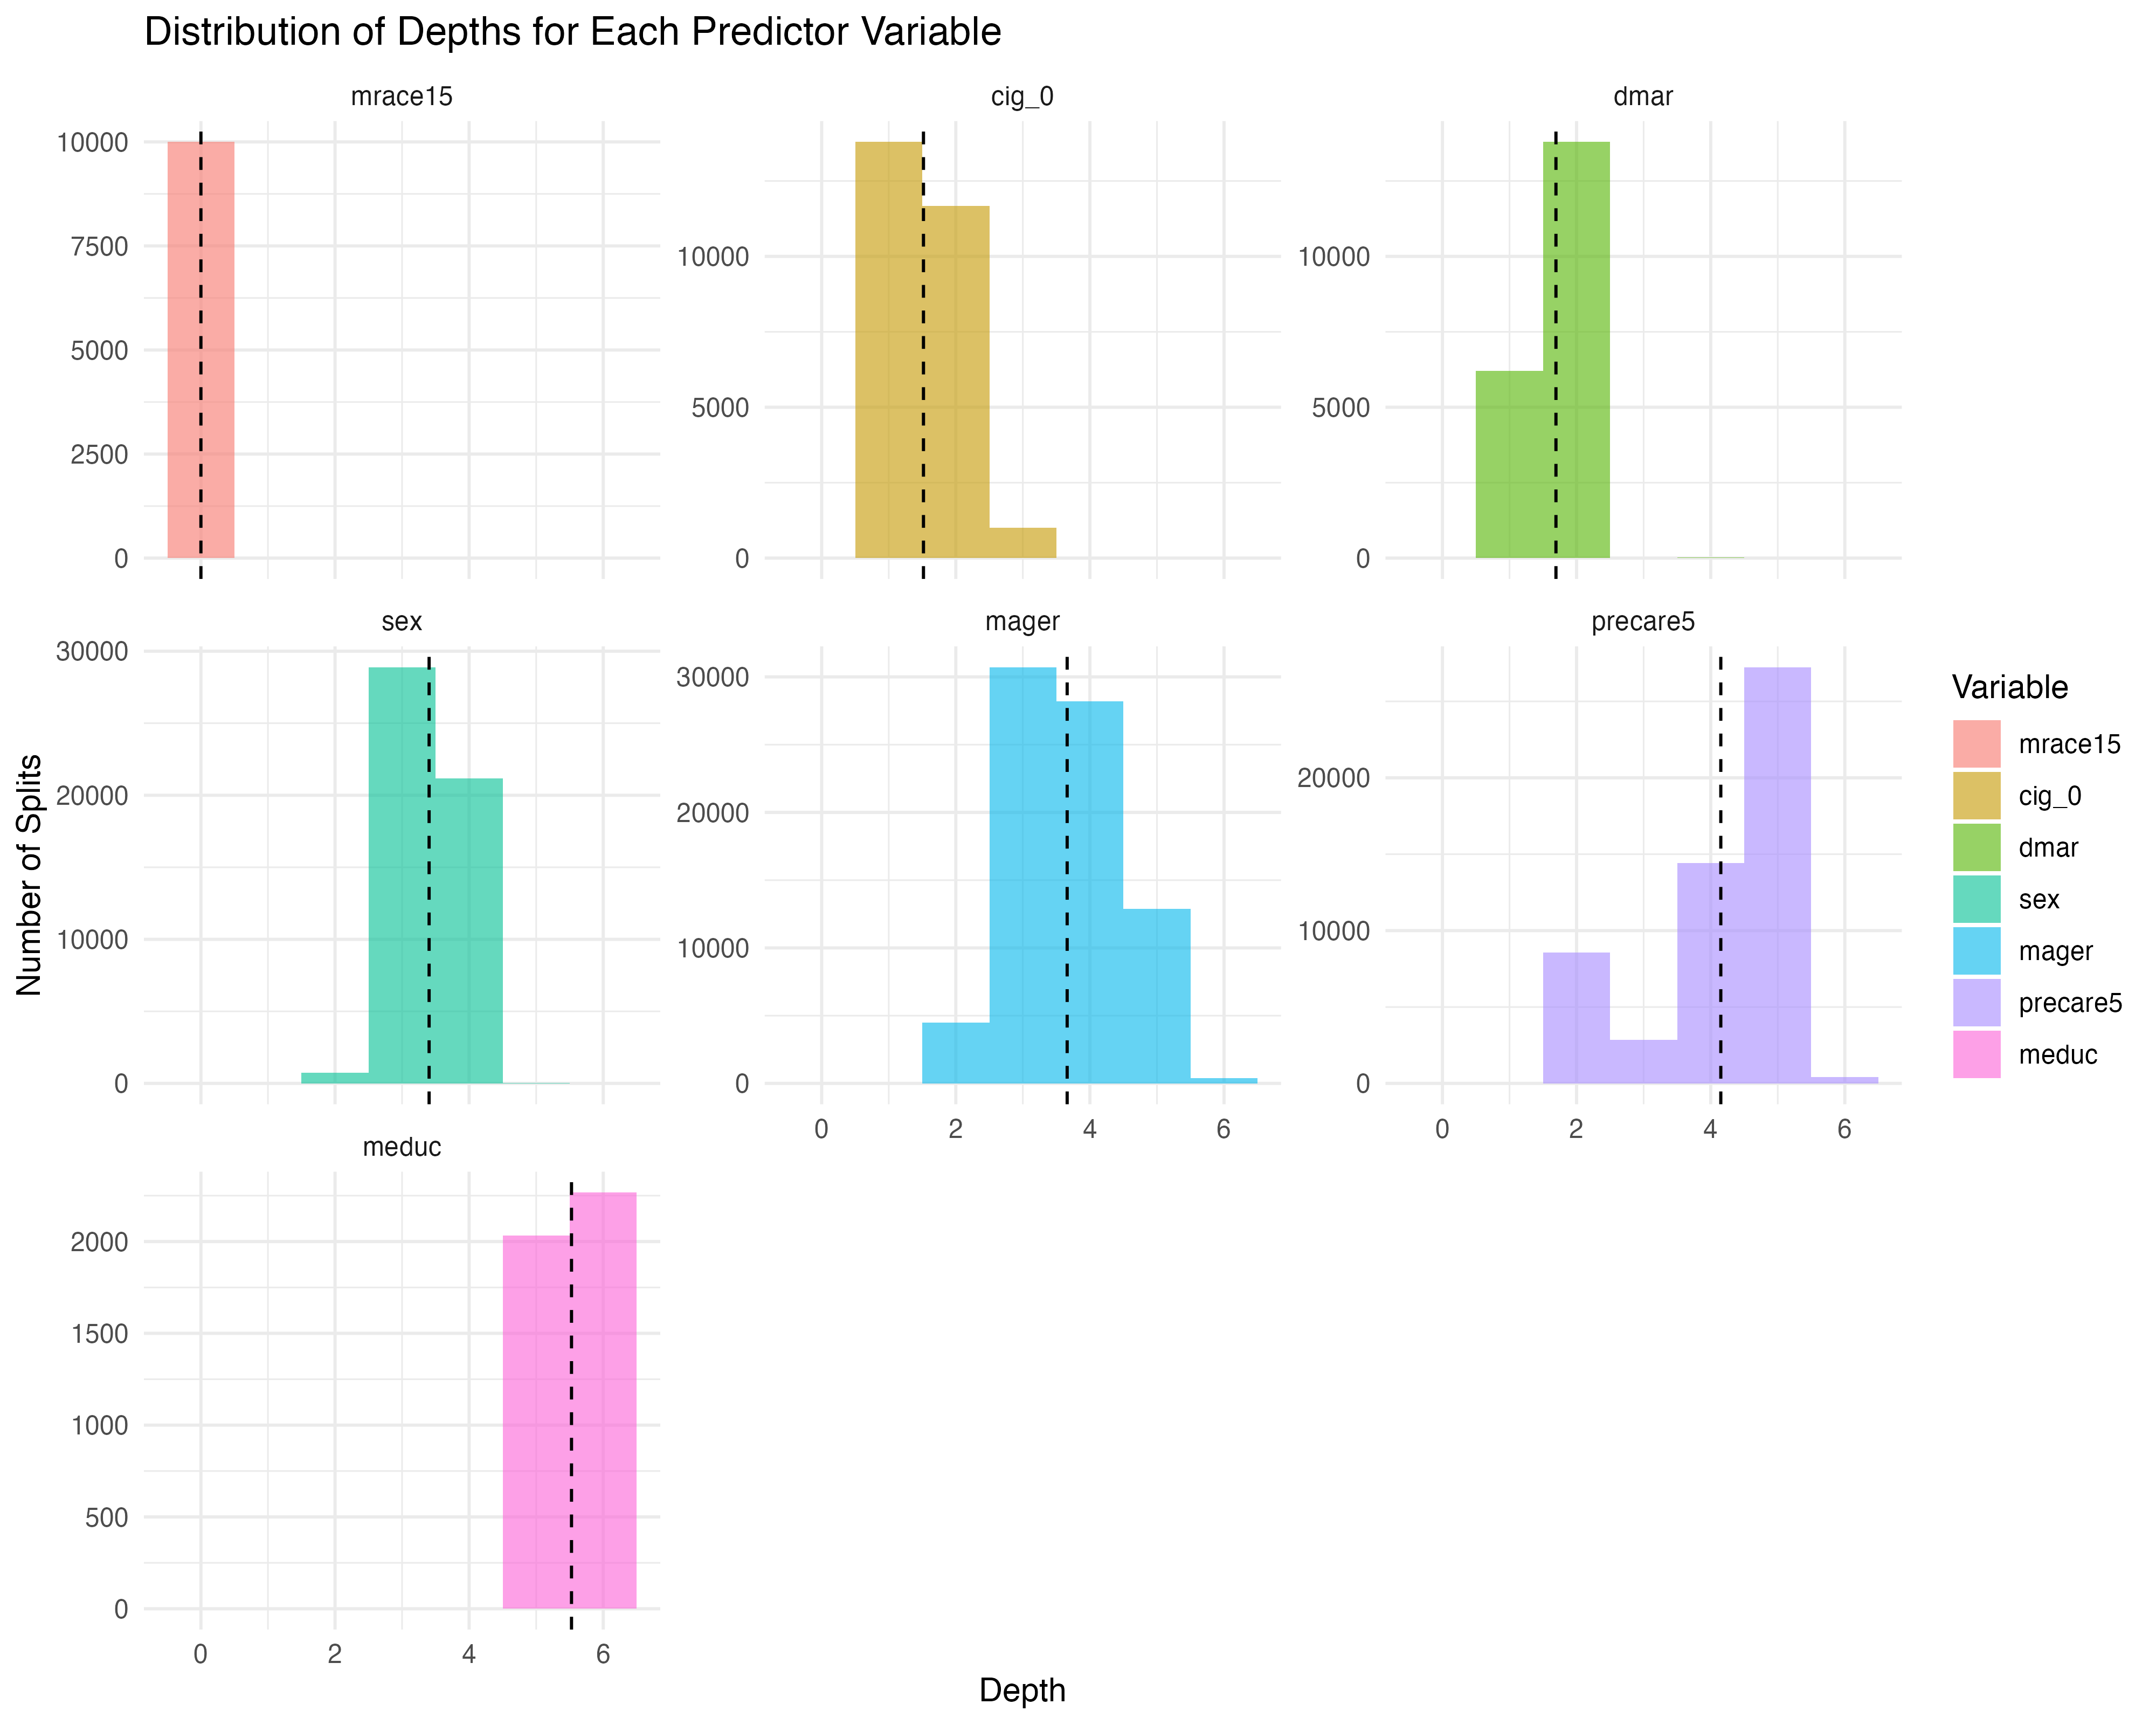
\includegraphics[width=\linewidth]{plots/depth_distributions.png}\\[-2pt]
    {\footnotesize Full model}
  \column{0.5\linewidth}
    \centering
    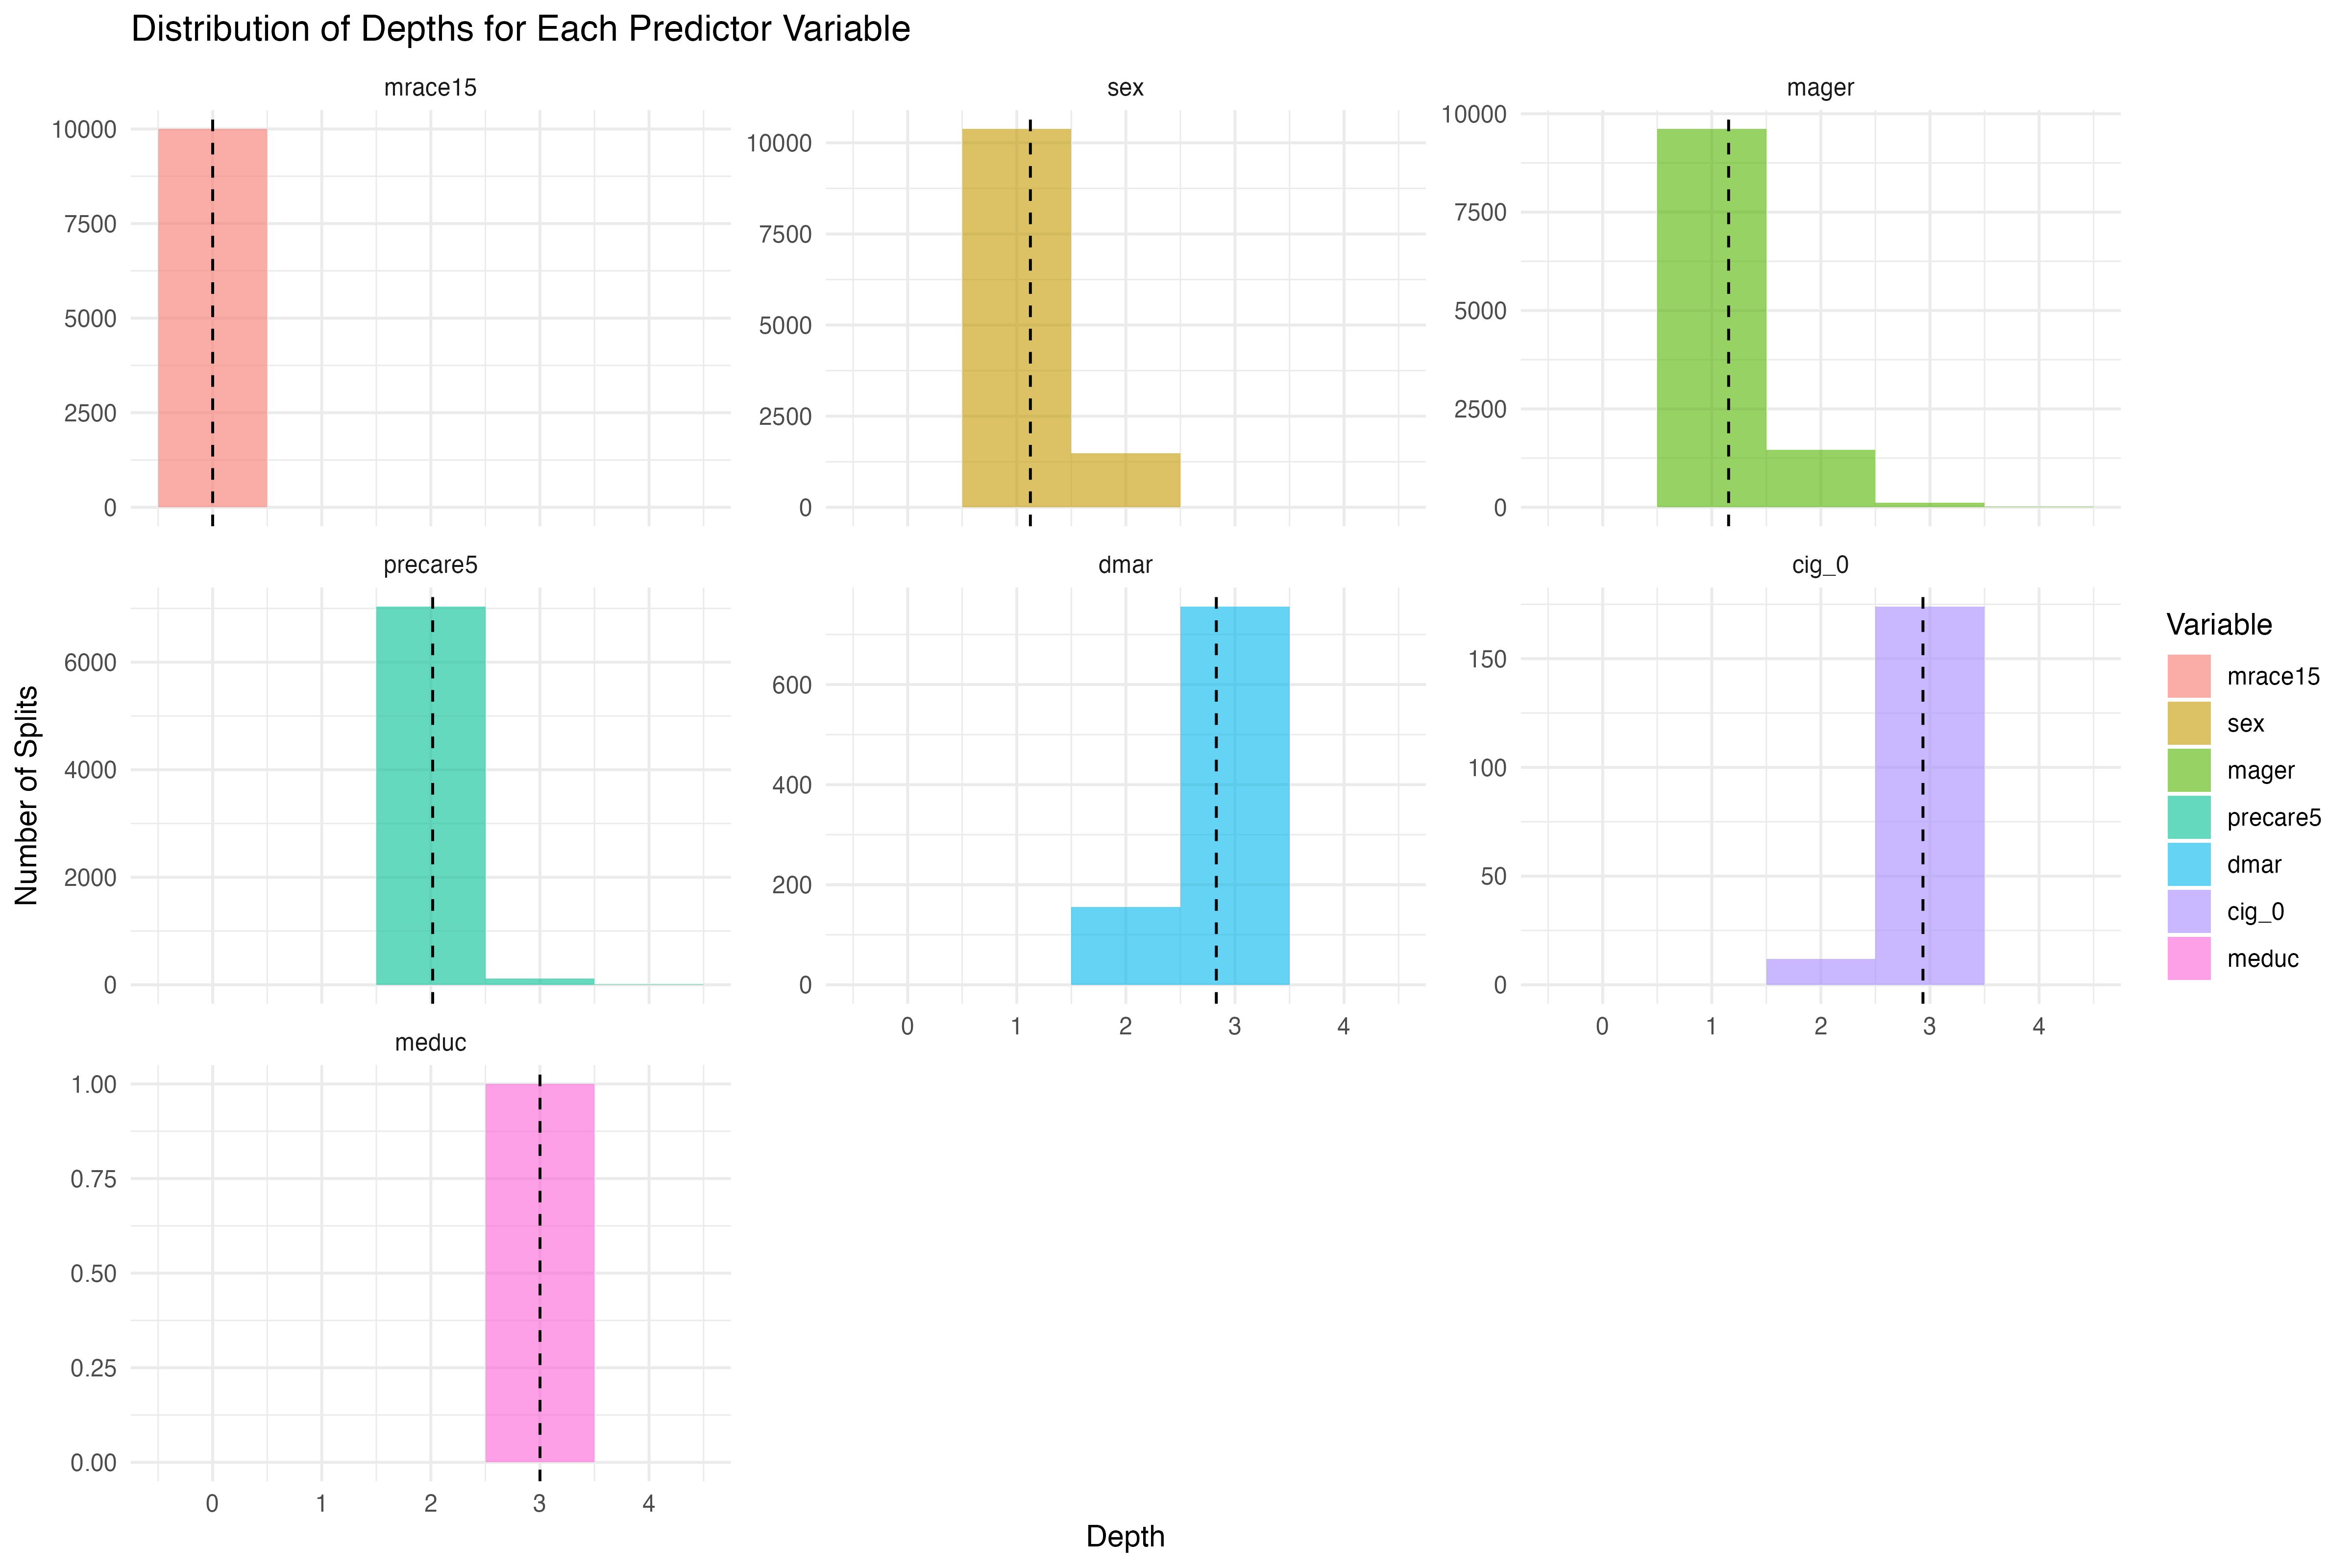
\includegraphics[width=\linewidth]{plots/depth_distributions_2.png}\\[-2pt]
    {\footnotesize LBW‑only model}
\end{columns}
\end{frame}


\begin{frame}{Bootstrap Probability Estimates by Risk Profile}
\small Aggregate mean $\hat{\pi}_{i,k}$ across $B=10,000$ bootstraps for \emph{high-risk} (class 69) and \emph{low-risk} (class 28) maternal profiles. Error bars show 95\% percentile intervals.

\begin{columns}[T]
  \column{0.42\linewidth}
    \centering
    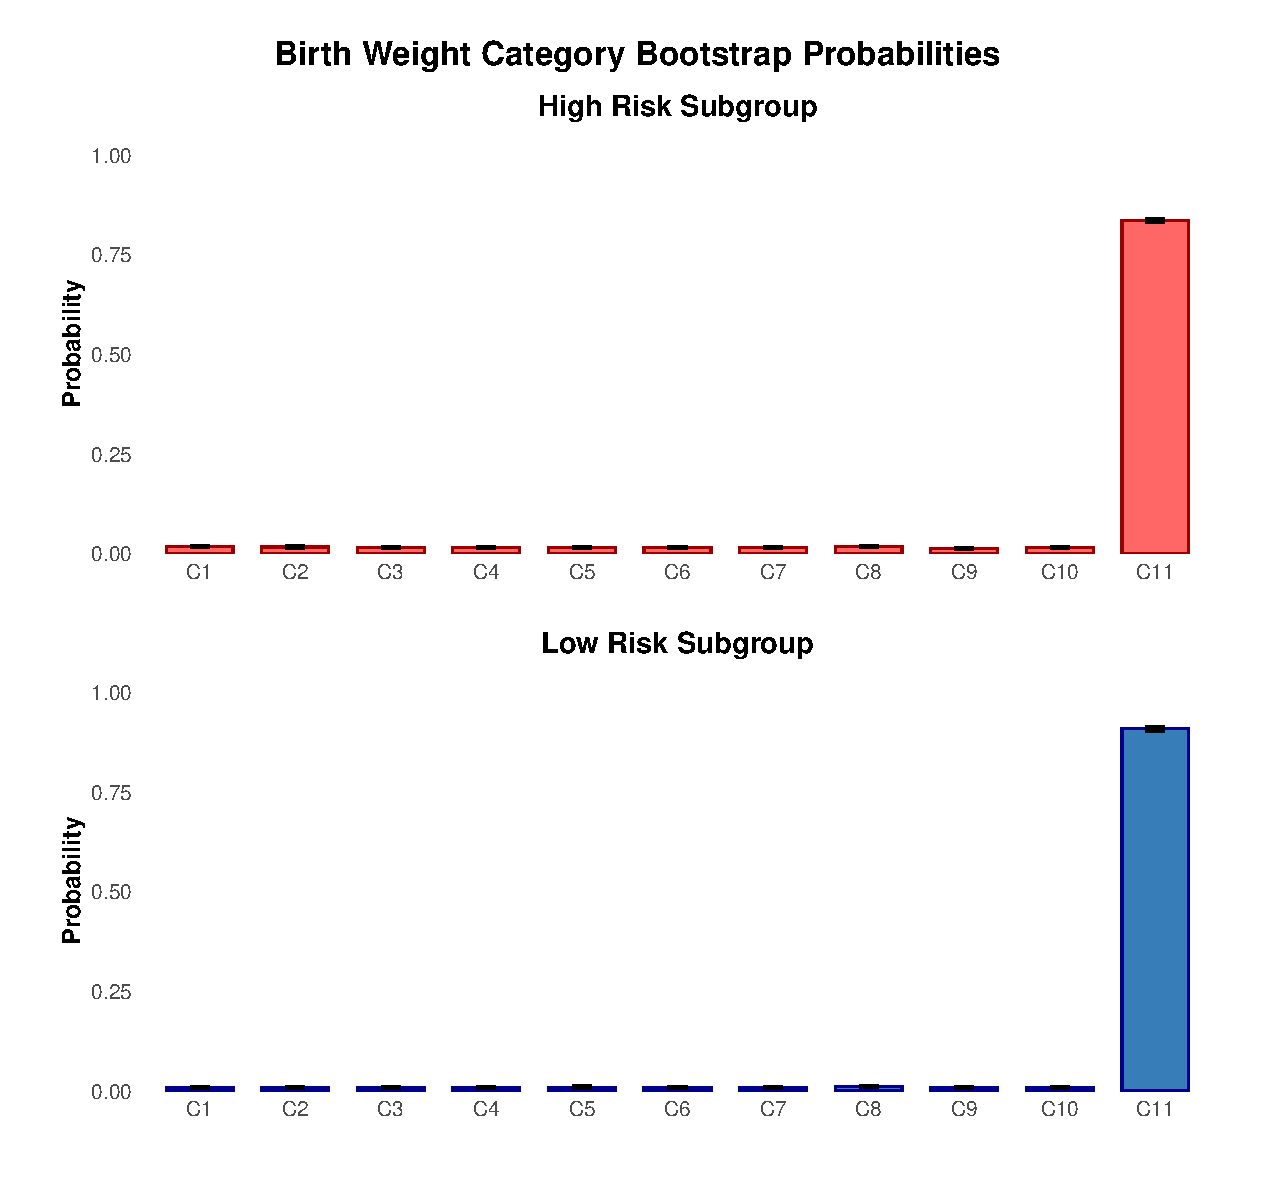
\includegraphics[width=\linewidth]{plots/high_low_risk_full.pdf}\\[-2pt]
    {\footnotesize Full model: $\pm \approx 0.002$}
  \column{0.42\linewidth}
    \centering
    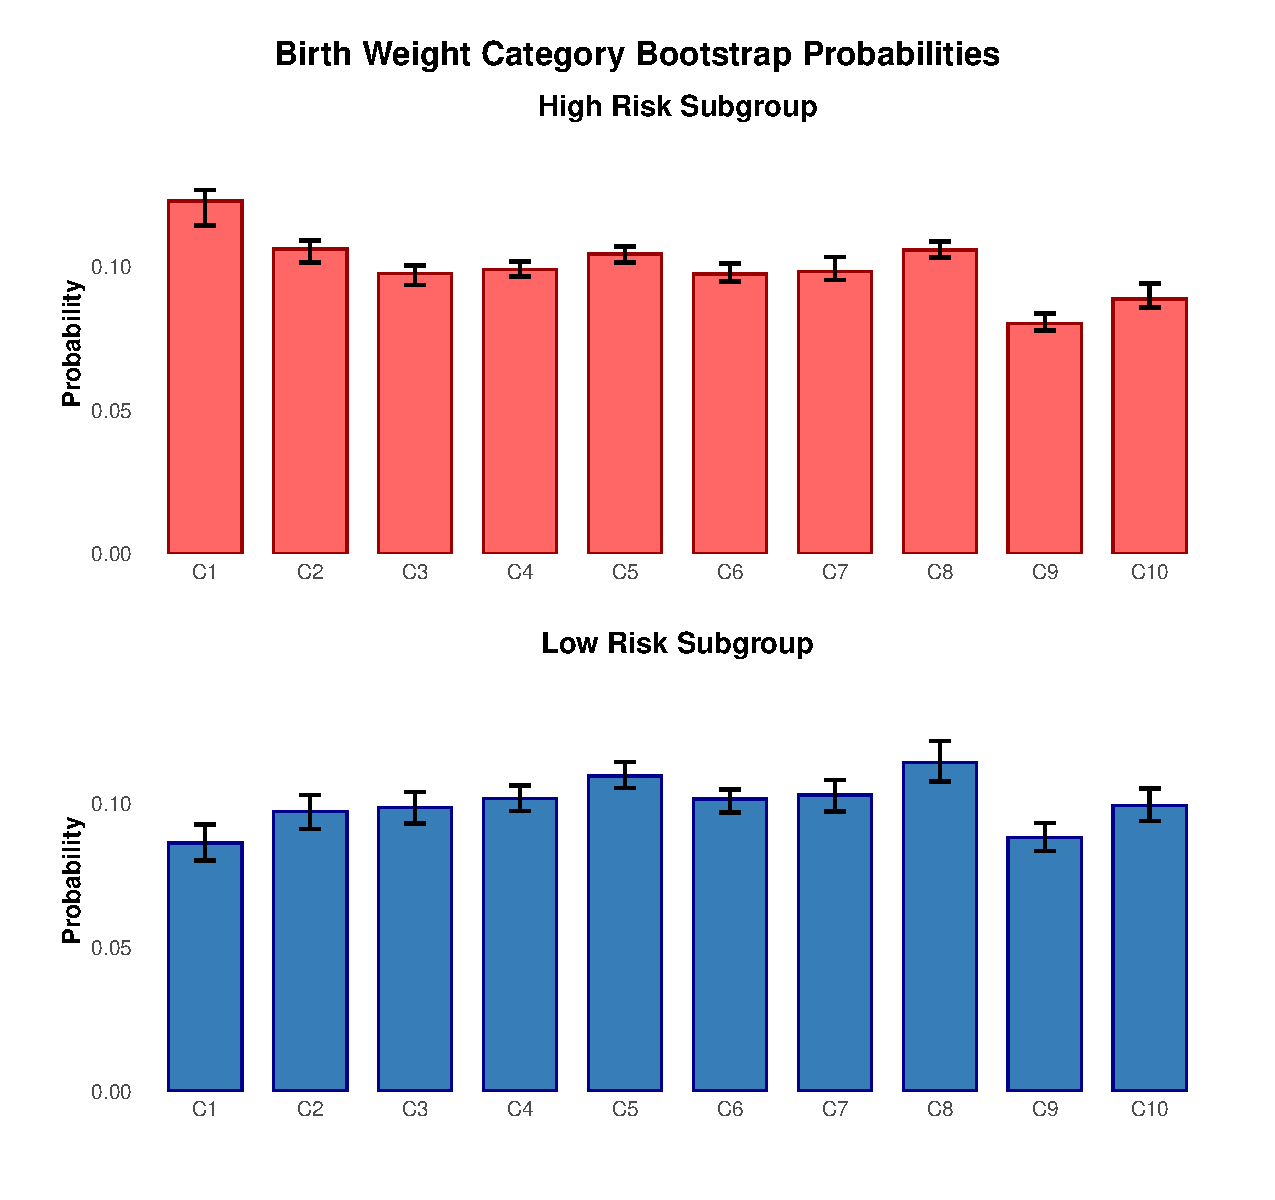
\includegraphics[width=\linewidth]{plots/high_low_risk_small.pdf}\\[-2pt]
    {\footnotesize LBW‑only model: $\pm \approx 0.008$}
\end{columns}
\end{frame}


% =========================================================
\section{Key Findings}

% \begin{frame}{Risk Subgroups}
% \begin{itemize}
%   \item \textbf{Highest risk}: Black, smoking, unmarried mothers \citep{smoking_lbw,kff_maternal_infant_health_a}.
%   \item \textbf{Lowest risk}: non-Black, non-smoking, married mothers of male infants.
%   \item Within LBW tail, infant sex and maternal age drive finer risk gradients \citep{decreasing_sex_diff_birth_weight2009,age_differences_lbw}.
% \end{itemize}
% \end{frame}

% % ───────────────────────────────────────────────────────────
% \begin{frame}{Risk Stratification Highlights}
% \begin{itemize}
%   \item \textbf{High‑risk} (class 69) $\Rightarrow$ NBW probability 83.6\% (7\% lower than baseline); extreme‑LBW risk \(\times2\) for high-risk profile.
%   \item \textbf{Low‑risk} (class 28): 
%   \item Within the LBW tail, finer gradients are driven by infant sex (female $>$ male), young maternal age, and inadequate prenatal care.
% \end{itemize}
% \end{frame}

% ───────────────────────────────────────────────────────────
\begin{frame}{Predictor Importance \& Risk Across 10\,000 Bootstrap Trees}
\begin{itemize}
  \item \textbf{Full model}
        \begin{itemize}
            \item Race, smoking, marital status selected in \emph{every} tree and dominate root splits.
            \item Prenatal care \& maternal age enter later; education appears in 38\% of trees at deep nodes.
            \item High-risk vs. low-risk NBW estimates reduced by 7\% (83.6\% vs. 90.9\%).
            \item Clear disadvantage in high-risk profile. For most severe BW category, probability estimates are more than twice as large (1.9\% vs. 0.8\%)
        \end{itemize}
  \item \textbf{LBW‑only model}
        \begin{itemize}
            \item Race and infant gender selected in every tree; maternal age in 97\% of trees.
            \item Socioeconomic predictors (marital, smoking, education) rarely/never chosen ($<$10\%).
            \item High-risk profile reflect higher severe LBW estimates, while low-risk profile reflect less severe estimates.
        \end{itemize}
  % \item Predictor hierarchy is stable under depth limits (2–5) and two‑tier parametric bootstrapping.
\end{itemize}
\end{frame}

% =========================================================
\section{Methodological Contributions}

\begin{frame}{Methodological Contributions}
\small
\begin{itemize}
  \item \textbf{DM–CART integration}: Dirichlet–Multinomial impurity brings Bayesian smoothing into CART, eliminating zero‑cell counts while retaining strong interpretability.
  \item \textbf{Informed priors from 2020 data}: quantile information for binning the 2021 data creates stable and informed Dirichlet prior based on historic data.
  \item \textbf{Two‑tier parametric bootstrap}: ensures variability in the consolidated counts data.
\end{itemize}
\end{frame}



% =========================================================
\section{Conclusions \& Future Work}

\begin{frame}{Conclusions}
\small
\begin{itemize}
    \item \textbf{Model focus}: Socioeconomic/demographic information used in full model to contrast diverse BW outcomes. LBW-only model shifts focus on biological/genetic predictors. 
  \item \textbf{Key risk factors}: maternal race, smoking, and marital status dominate full model; infant sex, maternal age, and prenatal care refine LBW risk.
  \item \textbf{Model performance:} DM-CART delivers clear, actionable subgroup rules that align with epidemiological literature and remain robust across 10,000 bootstrap replicates.  
  \item \textbf{Generalizability:} the Bayesian tree framework is extensible to other high-dimensional multinomial-count problems.
\end{itemize}
\end{frame}

% ---------- LIMITATIONS ----------
\begin{frame}{Limitations}
\small
\begin{itemize}
  \item Reductionist encoding of predictor variables; discarding key information about predictors.
  \item Race predictor is a very coarse proxy for other socioeconomic/demographic variables. These might be a better choice depending on modeling framework.
  \item Limited set of seven binary predictors simplifies the problem for the sake of interpretability.
  \item Analysis is cross‑sectional (2021) with no temporal trend.
\end{itemize}
\end{frame}

\begin{frame}{Future Directions}
\small
\begin{itemize}
  \item \textbf{Richer maternal‑health features}: hypertension, diabetes, BMI, mental‑health, prior pregnancy complications.
  \item \textbf{Contextual variables}: air quality, housing \& food access, neighborhood crime, proximity to prenatal services.
  \item \textbf{Temporal modeling}: introduce multi‑year trends to analyze BW outcomes.
  \item \textbf{Clinical deployment}: embed a risk calculator into EHR workflows; practitioner usage for clinical risk assessment.
\end{itemize}
\end{frame}

% ---------------------------------------------------------
\begin{frame}{Acknowledgments}
\small 
\begin{itemize}
  \item \textbf{Advisors:} Dr. P. Richard Hahn (advisor), Dr.  Shuang Zhou, Dr. Shiwei Lan 
  \item \textbf{Personal support:} family, friends, and medical team at PCH.
\end{itemize}
\end{frame}

% ---------- Thank-you ----------
\begin{frame}[plain]
  \centering\Huge Thank you!\\[1ex]\Large Questions?
\end{frame}

% ---------- References ----------
\begin{frame}[allowframebreaks]{References}
\footnotesize
\bibliography{references}
\end{frame}


\end{document}